%%%%%%%%%%%%%%%%%%%%%%%%%%%%%%%%%%%%%%%%%%%%%%%%%%%%%%%%%%%%%%%%%%%%%%%%%%%%%%%%%%
\begin{frame}[fragile]\frametitle{}
\begin{center}
{\Large Linear Regression}
\end{center}
\end{frame}

%%%%%%%%%%%%%%%%%%%%%%%%%%%%%%%%%%%%%%%%%%%%%%%%%%%%%%%%%%%%%%%%%%%%%%%%
\begin{frame}[fragile]\frametitle{Want to know future? Predictions}
% How can I make predictions about real-world quantities?
\begin{itemize}
\item How does sales volume change with changes in price. 
\item How is this affected by changes in the weather?
\item How does the amount of a drug absorbed vary with dosage and with body weight of patient? 
\item Does it depend on blood pressure?
%\item How are the conversions on an ecommerce website affected by two different page titles in an A/B comparison?
%\item How does the energy released by an earthquake vary with the depth of it's epicenter?
%\item How is the interest rate charged on a loan affected by credit history and by loan amount?
\end{itemize}
Answering questions like these, requires us to create a model.
\end{frame}

%%%%%%%%%%%%%%%%%%%%%%%%%%%%%%%%%%%%%%%%%%%%%%%%%%%%%%%%%%%%%%%%%%%%%%%%
\begin{frame}[fragile]\frametitle{The model}
\begin{itemize}
\item A model is a formula where one variable (response) varies depending on one or more independent variables (covariates). 
\item The formula (model) can be simple or complex.
%\item For the loan example, interest rate might depend on FICO score, state, loan amount, and loan duration amongst others.
\item Simplest is a Linear Model where the dependent varies linearly with the independent variable(s).
\item Creating a Linear Model involves a technique known as Linear Regression.
\end{itemize}
\end{frame}

%%%%%%%%%%%%%%%%%%%%%%%%%%%%%%%%%%%%%%%%%%%%%%%%%%%%%%%%%%%%%%%%%%%%%%%%
\begin{frame}[fragile]\frametitle{Remember? - High School Physics Lab}
\begin{itemize}
\item Finding how acceleration changes when Force is applied
\item For some input X (say force), got output Y (say acceleration).
\item Plotted the pairs of observations x, y.
\end{itemize}
\begin{center}
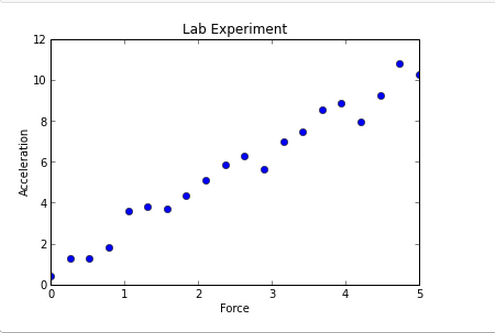
\includegraphics[width=0.45\linewidth]{lab1}
\end{center}
What next?
\end{frame}

%%%%%%%%%%%%%%%%%%%%%%%%%%%%%%%%%%%%%%%%%%%%%%%%%%%%%%%%%%%%%%%%%%%%%%%%
\begin{frame}[fragile]\frametitle{Fitting line}
\begin{itemize}
\item Then you had to fit a straight line through points
\item A visual ``best fit'', some points above, some below.
\item Found'm' the slope (how?), and 'b' (how?). 
\end{itemize}
\begin{center}
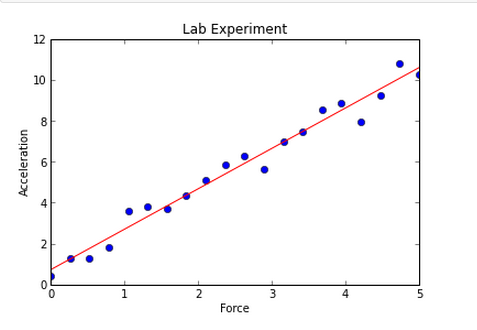
\includegraphics[width=0.45\linewidth]{lab2}
\end{center}
Whats the model here?
\end{frame}


%%%%%%%%%%%%%%%%%%%%%%%%%%%%%%%%%%%%%%%%%%%%%%%%%%%%%%%%%%%%%%%%%%%%%%%%
\begin{frame}[fragile]\frametitle{Fitting line}
\begin{itemize}
\item Equation of line, the formula, itself is the model.
\item You were doing informal Linear Regression.
\end{itemize}
\begin{center}
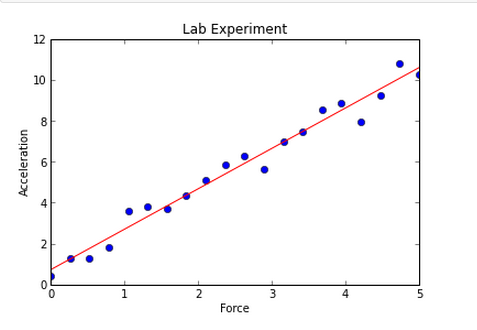
\includegraphics[width=0.45\linewidth]{lab2}
\end{center}
\end{frame}


%%%%%%%%%%%%%%%%%%%%%%%%%%%%%%%%%%%%%%%%%%%%%%%%%%%%%%%%%%%%%%%%%%%%%%%%
\begin{frame}[fragile]\frametitle{Linear Regression}
\begin{itemize}
\item What: for predicting a quantitative variable
\item Age: ``it's been around for a long time''. The term regression was devised by Francis Galton in his article 
Regression Towards Mediocrity in Hereditary Stature in 1886. 
\item Complexity: easy to understand and use
\item Popularity: still widely used
\end{itemize}
%Fancier, modern, data mining approaches can be seen as generalization or extensions of Linear Regression.
\end{frame}


%%%%%%%%%%%%%%%%%%%%%%%%%%%%%%%%%%%%%%%%%%%%%%%%%%%%%%%%%%%%%%%%%%%%%%%%
\begin{frame}[fragile]\frametitle{Possible Techniques}
\begin{itemize}
\item Statisticians know Regression as OLS (Ordinary Least Square) method to fit a line.  Deals with minimization of RMS (Root Mean Square) error.
\item Theoretical/Analytical Solution $W = (X^TX)^{-1} X^T y$. Not practical for large matrices. Also, matrix is not invertible if any two rows are same.
\item Machine Learning Engineers know Regression as prediction of continuous variables (floats). It uses Gradient Descent for the minimization part.
\end{itemize}
%Fancier, modern, data mining approaches can be seen as generalization or extensions of Linear Regression.
\end{frame}

%%%%%%%%%%%%%%%%%%%%%%%%%%%%%%%%%%%%%%%%%%%%%%%%%%%%%%%%%%%%%%%%%%%%%%%%%%%%%%%%%%
\begin{frame}[fragile]\frametitle{}
\begin{center}
{\Large Linear Regression - Analytical Approach (OLS)}
\end{center}
\end{frame}



%%%%%%%%%%%%%%%%%%%%%%%%%%%%%%%%%%%%%%%%%%%%%%%%%%%%%%%%%%%%%%%%%%%%%%%%
\begin{frame}[fragile]\frametitle{Example: Tip Amount}
\begin{itemize}
\item In a restaurant, tip you pay to the waiter, 
\item Typically depends on the bill amount.
\item Smaller the bill, lesser the tip, and vice versa.
\end{itemize}

Can we predict the tip amount just by looking at the bill amount?

Inputs?

Outputs?
\end{frame}

%%%%%%%%%%%%%%%%%%%%%%%%%%%%%%%%%%%%%%%%%%%%%%%%%%%%%%%%%%%%%%%%%%%%%%%%
\begin{frame}[fragile]\frametitle{Example: Tip Amount}
\begin{itemize}
\item You collect, random (meaning, any) 6 tips.
\item YOU HAVE NOT COLLECTED THE BILL AMOUNT.
\item Just one variable (Meal id is just the descriptor its not a independent variable)
\item Any guesses?
\end{itemize}
\end{frame}

%%%%%%%%%%%%%%%%%%%%%%%%%%%%%%%%%%%%%%%%%%%%%%%%%%%%%%%%%%%%%%%%%%%%%%%%
\begin{frame}[fragile]\frametitle{Most Basic Situation}
\begin{center}
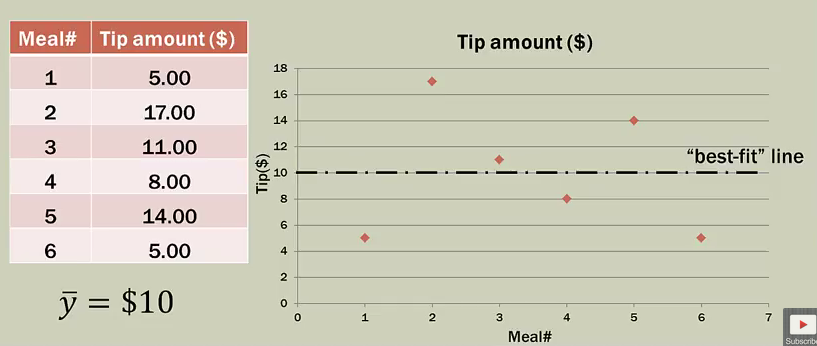
\includegraphics[width=0.9\linewidth]{linregf1}
\end{center}
\begin{itemize}
\item With just one variable, mean is the best we can do.
\item Note: not a single point falls on it.
\item Its just an estimate.
\item Goodness of fit?
\end{itemize}
\tiny{(Reference: Simple Linear Regression: Step-By-Step - Dan Wellisch)}
\end{frame}

%%%%%%%%%%%%%%%%%%%%%%%%%%%%%%%%%%%%%%%%%%%%%%%%%%%%%%%%%%%%%%%%%%%%%%%%
\begin{frame}[fragile]\frametitle{Example: Tip Amount}
\begin{center}
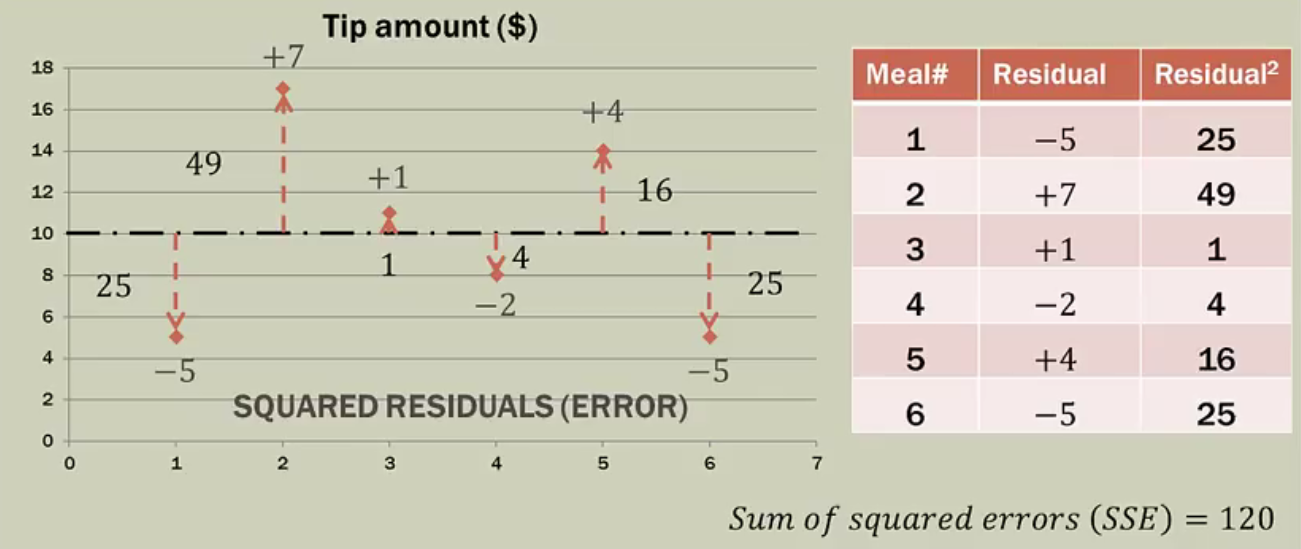
\includegraphics[width=0.9\linewidth]{linregf2}
\end{center}
\begin{itemize}
\item Std Variation says about goodness of fit.
\item Diff of each point with mean are called `residuals' or `errors'
\item Idea is to minimize SSE (Sum of Squared Errors) or RSS (Residual Sum of Squares)
\end{itemize}
\end{frame}

%%%%%%%%%%%%%%%%%%%%%%%%%%%%%%%%%%%%%%%%%%%%%%%%%%%%%%%%%%%%%%%%%%%%%%%%
\begin{frame}[fragile]\frametitle{Important Concept}
\begin{center}
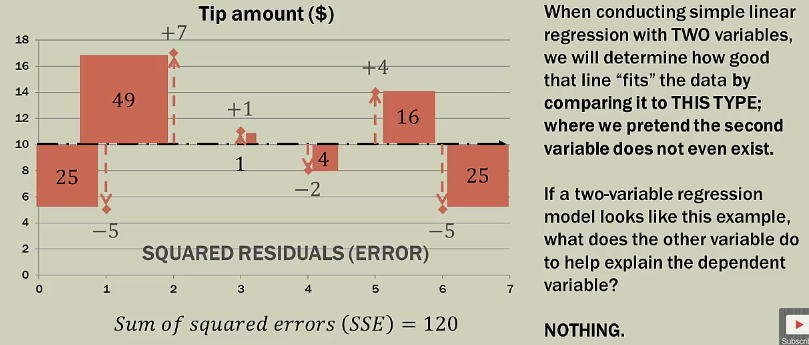
\includegraphics[width=0.9\linewidth]{linregf3}
\end{center}
\begin{itemize}
\item With just the target variable (tips) we got SSE as 120.
\item If we add one more variable to the problem, ie bill amount, what do you expect of SSE?
\item It should reduce, or else, whats the use of adding this variable.
\item So, we will compare our Linear regression fit line with this (one variable) line.
%\item Simple Linear regression is part of Bivariate statistics, ie of two variables, eg Covariance, Correlation
\end{itemize}
\end{frame}

%%%%%%%%%%%%%%%%%%%%%%%%%%%%%%%%%%%%%%%%%%%%%%%%%%%%%%%%%%%%%%%%%%%%%%%%
\begin{frame}[fragile]\frametitle{Important Concept}
\begin{center}
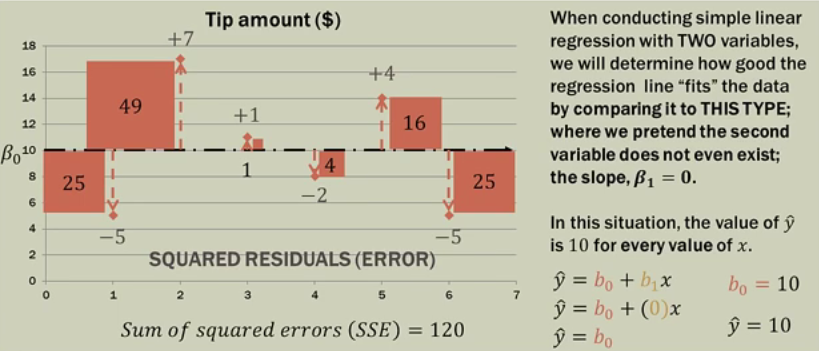
\includegraphics[width=0.9\linewidth]{linregf4}
\end{center}
\begin{itemize}
%\item Simple Linear regression is part of Bivariate statistics, ie of two variables, eg Covariance, Correlation
\item We find slope and intercept as $b_1$ and $b_0$ respectively.
\item A line with $b_1 = 0$ is the horizontal line.
\item Its SSE becomes the benchmark. Any selected pair of $b_1$ and $b_0$ should give SSE less than the benchmark SSE.
\end{itemize}
\end{frame}

%%%%%%%%%%%%%%%%%%%%%%%%%%%%%%%%%%%%%%%%%%%%%%%%%%%%%%%%%%%%%%%%%%%%%%%%
\begin{frame}[fragile]\frametitle{Linear Regression with Two Variables}
\begin{center}
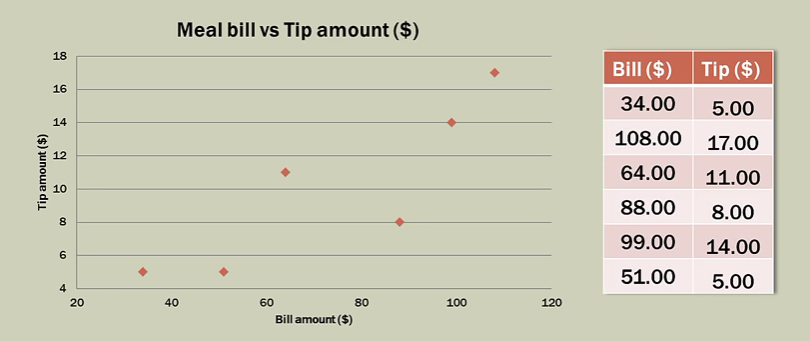
\includegraphics[width=0.9\linewidth]{linregf5}
\end{center}
\begin{itemize}
\item You can fit a line, however you want.
\item Even horizontal line can be put
\item But then, which one is the best?
\item Need to be at least better than horizontal line!!
\end{itemize}
\end{frame}

%%%%%%%%%%%%%%%%%%%%%%%%%%%%%%%%%%%%%%%%%%%%%%%%%%%%%%%%%%%%%%%%%%%%%%%%
\begin{frame}[fragile]\frametitle{Methodology}
Hypothesis: A line passing through the centroid of the data points will be good. Lets check.

\begin{center}
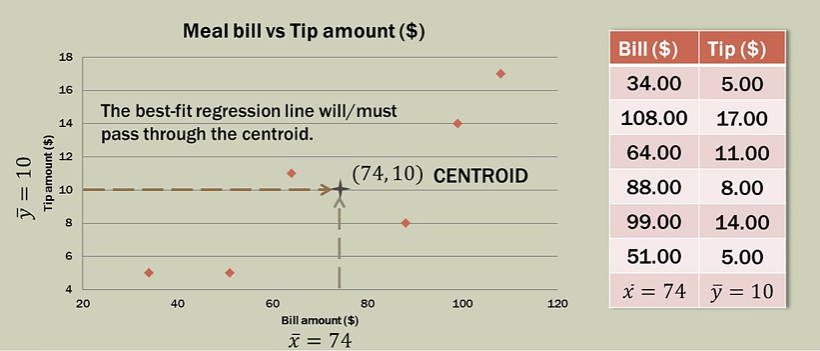
\includegraphics[width=0.9\linewidth]{linregf6}
\end{center}
\begin{itemize}
\item Calculate mean of both x and y.
\item Line needs to pass through this point
\end{itemize}
\end{frame}

%%%%%%%%%%%%%%%%%%%%%%%%%%%%%%%%%%%%%%%%%%%%%%%%%%%%%%%%%%%%%%%%%%%%%%%%
\begin{frame}[fragile]\frametitle{Calculations}
\begin{center}
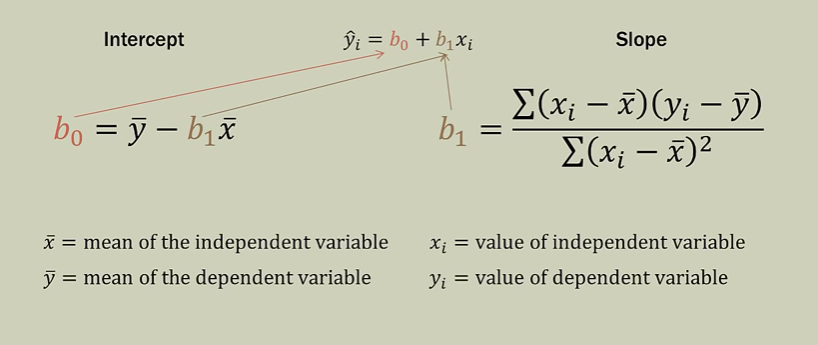
\includegraphics[width=0.9\linewidth]{linregf7}
\end{center}
\begin{itemize}
\item Intercept and Slope are calculated as above.
\item A simple tabular calculations can be done.
\end{itemize}
\end{frame}

%%%%%%%%%%%%%%%%%%%%%%%%%%%%%%%%%%%%%%%%%%%%%%%%%%%%%%%%%%%%%%%%%%%%%%%%
\begin{frame}[fragile]\frametitle{Calculations}
\begin{center}
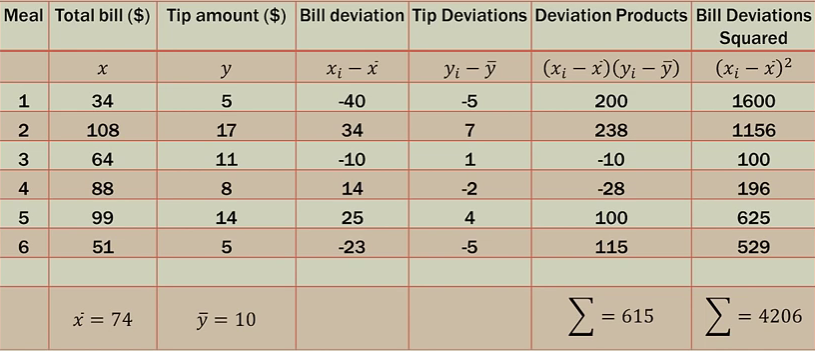
\includegraphics[width=\linewidth]{linregf8}
\end{center}
\begin{itemize}
\item Slope comes to $= 615/4206 = 0.1462$
\item Intercept comes to $= 10 - 0.1462(74) = -0.818$
\item So, eq is $y = 0.1462x - 0.8188$
\end{itemize}
\end{frame}


%%%%%%%%%%%%%%%%%%%%%%%%%%%%%%%%%%%%%%%%%%%%%%%%%%%%%%%%%%%%%%%%%%%%%%%%
\begin{frame}[fragile]\frametitle{Interpretation}
\begin{center}
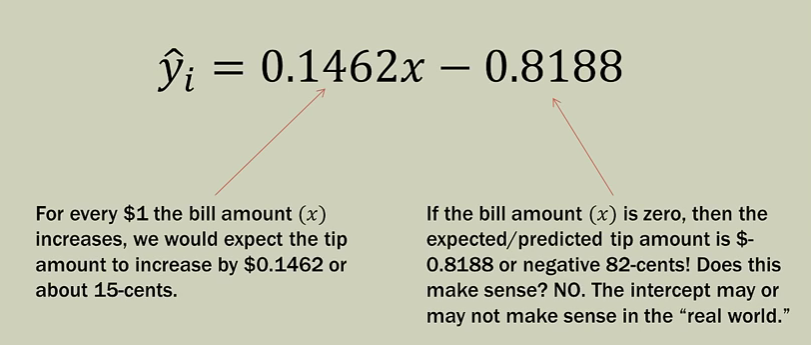
\includegraphics[width=0.9\linewidth]{linregf9}
\end{center}
\begin{itemize}
\item Slope gives proportionality with which tip is calculated.
\item Intercept may or may not make sense in real life.
\item Is this manual calculation giving good line?
\end{itemize}
\end{frame}

%%%%%%%%%%%%%%%%%%%%%%%%%%%%%%%%%%%%%%%%%%%%%%%%%%%%%%%%%%%%%%%%%%%%%%%%
\begin{frame}[fragile]\frametitle{Evaluation}
\begin{center}
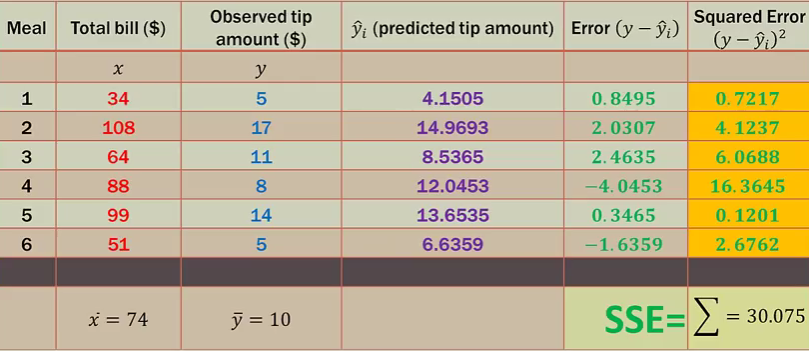
\includegraphics[width=0.9\linewidth]{linregf10}
\end{center}
\begin{itemize}
\item Sum of Squares of Error , SSE is 30 for our manual model
\item Its far less than the horizontal line benchmark of 120.
\item So, by adding Bill amount as independent variable, reduced error by about 90.
\end{itemize}
\end{frame}

%%%%%%%%%%%%%%%%%%%%%%%%%%%%%%%%%%%%%%%%%%%%%%%%%%%%%%%%%%%%%%%%%%%%%%%%
\begin{frame}[fragile]\frametitle{Evaluation}
\begin{center}
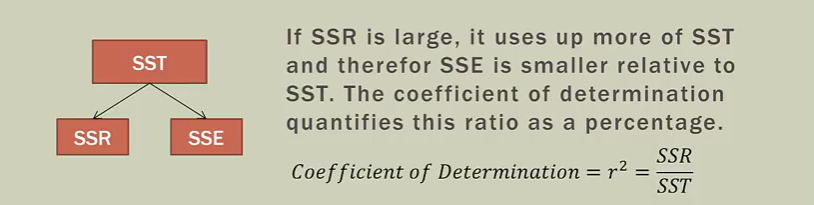
\includegraphics[width=0.9\linewidth]{linregf11}
\end{center}
\begin{itemize}
\item SST (sum of squares total) is the benchmark error. Its constant ie 120.
\item SSE (sum of squares error) is the level to which we could get error to it by applying regression ie 30.
\item The difference, the achievement by regression is called SSR (sum of squares by regression) ie 90.
%\item Coefficient of determination $r^2 = SSR/SST = 90/120 = 0.75$ Good fit.
\end{itemize}
\end{frame}

%%%%%%%%%%%%%%%%%%%%%%%%%%%%%%%%%%%%%%%%%%%%%%%%%%%%%%%%%%%%%%%%%%%%%%%%
\begin{frame}[fragile]\frametitle{Evaluation}
\begin{center}
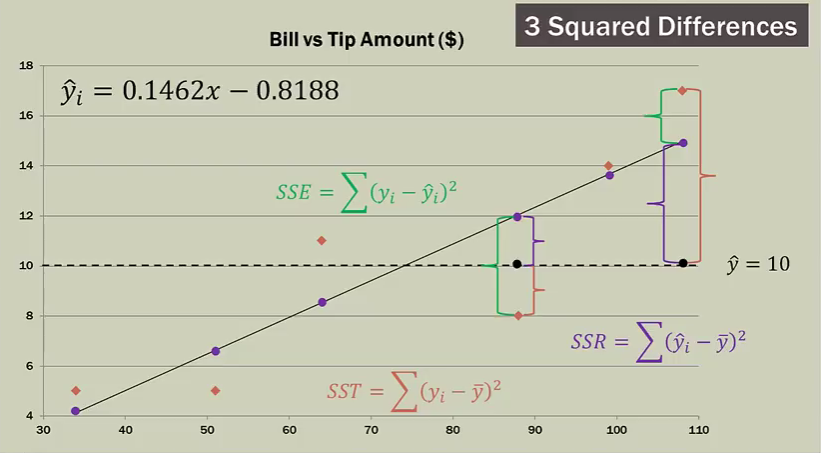
\includegraphics[width=0.9\linewidth]{linregf12}
\end{center}

% Some of the total variation in the data (distance from datapoint  to benchmark line, SST : $y_i$ to $\bar{y}$) is captured by 
 % the regression line (the distance from the regression line to benchmark line, SSR: $\hat{y_i}$ to $\bar{y}$) and
 % remaining by, the error (distance from the point to the regression line, SSE: $y_i$to $\hat{y_i}$)). 
\begin{itemize}
\item For each x, there is predicted y and actual y
\item 3 relationships: observed, predicted and total
% \item Sum of squares among them.
\item Can decide quality based on the ratios among them.
\end{itemize}
\end{frame}

%%%%%%%%%%%%%%%%%%%%%%%%%%%%%%%%%%%%%%%%%%%%%%%%%%%%%%%%%%%%%%%%%%%%%%%%
\begin{frame}[fragile]\frametitle{$R^2$ Statistics}
\begin{itemize}
\item $SST = SSR + SSE$

\item $SST$: Total variance in the response Y. Amount of variability inherent in the response, before the regression is performed. $y_i$ to $\bar{y}$
\item It has two components, one explained by this regression model, other the unexplained.
\item $SSR$: The amount of variability that is explained after performing the regression. $\hat{y_i}$ to $\bar{y}$
\item $SSE$ : The amount of variability that is left unexplained, that our model could not minimize. $y_i$to $\hat{y_i}$
%\item $R^2$ has an interpretational advantage over $RSE$

\end{itemize}
\end{frame}


% %%%%%%%%%%%%%%%%%%%%%%%%%%%%%%%%%%%%%%%%%%%%%%%%%%%%%%%%%%%%%%%%%%%%%%%%
% \begin{frame}[fragile]\frametitle{Derivation (optional)}

% \begin{align*}
% \sum (y_i - \bar{y})^2 &= \sum [ (y_i - \hat{y_i})  + ( \hat{y_i} - \bar{y} ) ] ^2 \\
% &= \sum  (y_i - \hat{y_i})^2  +  2 \sum (y_i - \hat{y_i})(\hat{y_i} - \bar{y})  + \sum ( \hat{y_i} - \bar{y} )^2 \\
% &= \sum  (y_i - \hat{y_i})^2  +  \sum ( \hat{y_i} - \bar{y} )^2 
% \end{align*}
% If $ 2 \sum (y_i - \hat{y_i})(\hat{y_i} - \bar{y}) = 0$ meaning  $2 \sum (y_i - \hat{y_i}) \hat{y_i} - \bar{y} \sum (y_i - \hat{y_i})$. Possible when:

% \begin{itemize}
% \item $e_i = (y_i - \hat{y_i})$ need to be orthogonal to fitted values so $ \sum (y_i - \hat{y_i}) \hat{y_i} = 0$
% \item The sum of the fitted values needs to be equal to the sum of the dependent variable  $ \sum y_i = \sum \hat{y_i}$
% \end{itemize}

% % % (Ref: https://stats.stackexchange.com/questions/207841/why-is-sst-sse-ssr-one-variable-linear-regression)
% \end{frame}


% %%%%%%%%%%%%%%%%%%%%%%%%%%%%%%%%%%%%%%%%%%%%%%%%%%%%%%%%%%%%%%%%%%%%%%%%
% \begin{frame}[fragile]\frametitle{$R^2$ Statistics}
% \begin{itemize}
% \item Coefficient of determination 
% $R^2 = \frac{SSR}{SST} = 1- \frac{SSE}{SST}$

% \item Advertising Dataset, $R^2 = 0.61$
% \item Just under two-thirds of the variability in sales is explained by a linear regression on TV.
% %\item $R^2$ has an interpretational advantage over $RSE$

% \end{itemize}
% \end{frame}

%%%%%%%%%%%%%%%%%%%%%%%%%%%%%%%%%%%%%%%%%%%%%%%%%%%%%%%%%%%%%%%%%%%%%%%%%
%\begin{frame}[fragile]\frametitle{$R^2$ Statistics}
%\begin{itemize}
%\item Proportion of variance
%$r^2 = \frac{SSR}{SST} = 1 - \frac{SSR}{SST}$ where, $SST = \sum (y_i - \bar{y})^2$ and  $SST = \sum (y_i - \hat{y_i})^2$
%\item $SST$: Total variance in the response Y. Amount of variability inherent in the response, before the regression is performed
%\item It has two components, one explained by this regression model, other the unexplained.
%\item $SSR$: amount of variability that is left unexplained after performing the regression
%\item $SST-SSR$ : the amount of variability that is explained
%\item Advertising Dataset, $r^2 = 0.61$
%\item Just under two-thirds of the variability in sales is explained by a linear regression on TV.
%%\item $R^2$ has an interpretational advantage over $RSE$
%
%\end{itemize}
%\end{frame}

%%%%%%%%%%%%%%%%%%%%%%%%%%%%%%%%%%%%%%%%%%%%%%%%%%%%%%%%%%%%%%%%%%%%%%%%%
%\begin{frame}[fragile]\frametitle{Making predictions about the future with supervised learning}
%\begin{itemize}
%\item The main goal in supervised learning is to learn a model from labeled training data 
%that allows us to make predictions about unseen or future data. 
%\item Here, the term 
%supervised refers to a set of samples where the desired output signals (labels) are 
%already known.
%\end{itemize}
%\end{frame}


% %%%%%%%%%%%%%%%%%%%%%%%%%%%%%%%%%%%%%%%%%%%%%%%%%%%%%%%%%%%%%%%%%%%%%%%%
% \begin{frame}[fragile]\frametitle{Linear Regression (Recap)}
% \begin{itemize}
% \item Used  to  estimate  real  values  (cost  of  houses, total  sales  etc.) 
% \item Establishes  relationship  between  independent  and  dependent variables by fitting a best line. 
% \item This best fit line is known as regression line and represented by a linear equation $Y= a *X + b$
% \item Can have one (simple) or multiple (multivariate) regression.
% \end{itemize}

% \end{frame}

% %%%%%%%%%%%%%%%%%%%%%%%%%%%%%%%%%%%%%%%%%%%%%%%%%%%%%%%%%%%%%%%%%%%%%%%%%%%%%%%%%%
% \begin{frame}[fragile]\frametitle{}
% \begin{center}
% {\Large Linear Regression - Ordinary Least Squares Approach}
% \end{center}
% \end{frame}

% %%%%%%%%%%%%%%%%%%%%%%%%%%%%%%%%%%%%%%%%%%%%%%%%%%%%%%%%%%%%%%%%%%%%%%%%
% \begin{frame}[fragile]\frametitle{Linear Regression}
% \begin{itemize}
% \item Linear regression can be represented as : $\large y_i = \sum_{j=0}^m w_j X_{ij} + \epsilon_i$
% \item One of the ways to calculate those weights is with the ordinary least squares method (OLS), which minimizes the mean squared error between the actual value of the dependent variable and the predicted value given by the model:
% $
% \begin{array}{rcl}\mathcal{L}\left(\textbf X, \textbf{y}, \textbf{w} \right) &=& \frac{1}{2n} \sum_{i=1}^n \left(y_i - \textbf{w}^\text{T} \textbf{x}_i\right)^2 \\
% &=& \frac{1}{2n} \left\| \textbf{y} - \textbf X \textbf{w} \right\|_2^2 \\
% &=& \frac{1}{2n} \left(\textbf{y} - \textbf X \textbf{w}\right)^\text{T} \left(\textbf{y} - \textbf X \textbf{w}\right)
% \end{array}
% $
% \end{itemize}

% \end{frame}

% %%%%%%%%%%%%%%%%%%%%%%%%%%%%%%%%%%%%%%%%%%%%%%%%%%%%%%%%%%%%%%%%%%%%%%%%
% \begin{frame}[fragile]\frametitle{Linear Regression}
% \begin{itemize}
% \item To solve this optimization problem, we need to calculate derivatives with respect to the model parameters. 
% \item We set them to zero and solve the resulting equation for $w$
% \end{itemize}

% \end{frame}


% %%%%%%%%%%%%%%%%%%%%%%%%%%%%%%%%%%%%%%%%%%%%%%%%%%%%%%%%%%%%%%%%%%%%%%%%
% \begin{frame}[fragile]\frametitle{Matrix differentiation Rules (recap)}
% $
% \begin{array}{rcl} 
% \frac{\partial}{\partial \textbf{X}} \textbf{X}^{\text{T}} \textbf{A} &=& \textbf{A} \\
% \frac{\partial}{\partial \textbf{X}} \textbf{X}^{\text{T}} \textbf{A} \textbf{X} &=& \left(\textbf{A} + \textbf{A}^{\text{T}}\right)\textbf{X} \\
% \frac{\partial}{\partial \textbf{A}} \textbf{X}^{\text{T}} \textbf{A} \textbf{y} &=&  \textbf{X}^{\text{T}} \textbf{y}\\
% \frac{\partial}{\partial \textbf{X}} \textbf{A}^{-1} &=& -\textbf{A}^{-1} \frac{\partial \textbf{A}}{\partial \textbf{X}} \textbf{A}^{-1} 
% \end{array}
% $

% \end{frame}

% %%%%%%%%%%%%%%%%%%%%%%%%%%%%%%%%%%%%%%%%%%%%%%%%%%%%%%%%%%%%%%%%%%%%%%%%
% \begin{frame}[fragile]\frametitle{Matrix differentiation for Variance Function}
% $
% \begin{array}{rcl} \frac{\partial \mathcal{L}}{\partial \textbf{w}} &=& \frac{\partial}{\partial \textbf{w}} \frac{1}{2n} \left( \textbf{y}^{\text{T}} \textbf{y} -2\textbf{y}^{\text{T}} \textbf{X} \textbf{w} + \textbf{w}^{\text{T}} \textbf{X}^{\text{T}} \textbf{X} \textbf{w}\right) \\
% &=& \frac{1}{2n} \left(-2 \textbf{X}^{\text{T}} \textbf{y} + 2\textbf{X}^{\text{T}} \textbf{X} \textbf{w}\right)
% \end{array}
% $
% $
 % \begin{array}{rcl} \frac{\partial \mathcal{L}}{\partial \textbf{w}} = 0 &\Leftrightarrow& \frac{1}{2n} \left(-2 \textbf{X}^{\text{T}} \textbf{y} + 2\textbf{X}^{\text{T}} \textbf{X} \textbf{w}\right) = 0 \\
% &\Leftrightarrow& -\textbf{X}^{\text{T}} \textbf{y} + \textbf{X}^{\text{T}} \textbf{X} \textbf{w} = 0 \\
% &\Leftrightarrow& \textbf{X}^{\text{T}} \textbf{X} \textbf{w} = \textbf{X}^{\text{T}} \textbf{y} \\
% &\Leftrightarrow& \textbf{w} = \left(\textbf{X}^{\text{T}} \textbf{X}\right)^{-1} \textbf{X}^{\text{T}} \textbf{y}
% \end{array}
% $


% These give optimized weights for which Variance is minimal.
% \end{frame}


%%%%%%%%%%%%%%%%%%%%%%%%%%%%%%%%%%%%%%%%%%%%%%%%%%%%%%%%%%%%%%%%%%%%%%%%%%%%%%%%%%
\begin{frame}[fragile]\frametitle{}
\begin{center}
{\Large Linear Regression - Machine Learning Approach}
\end{center}
\end{frame}


%%%%%%%%%%%%%%%%%%%%%%%%%%%%%%%%%%%%%%%%%%%%%%%%%%%%%%%%%%%
\begin{frame}[fragile]\frametitle{Linear regression}
	\begin{itemize}
	\item We have multiple observations of inputs and an output
	\item Object: to find a model, ie a formulation, adhering to more or less all data points
	\item ie. to attempt to find the ``best'' line
	\item But, which line is the ``best''?
	\item The horizontal line is the worst, the benchmark. We need to beat that!!
	\end{itemize}
	
\begin{center}
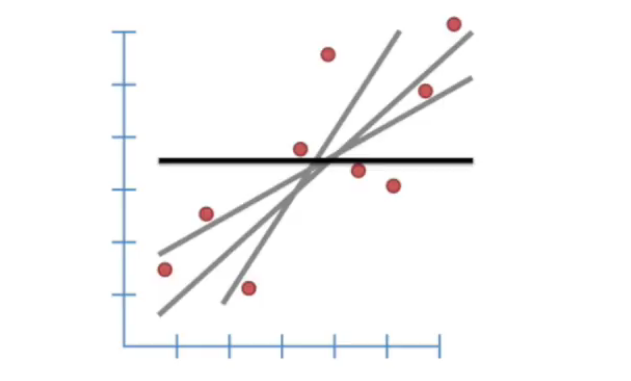
\includegraphics[width=0.5\linewidth,keepaspectratio]{statq58}
\end{center}
	
\tiny{(Ref: StatQuest: Linear Models - Josh Starmer )}	
\end{frame}

%%%%%%%%%%%%%%%%%%%%%%%%%%%%%%%%%%%%%%%%%%%%%%%%%%%%%%%%%%%
\begin{frame}[fragile]\frametitle{Sum of Squared Errors for Benchmark Line}
	
\begin{center}
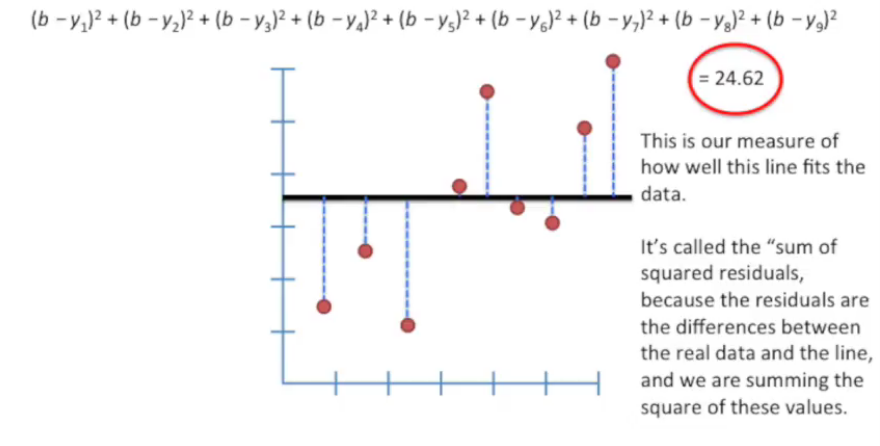
\includegraphics[width=0.8\linewidth,keepaspectratio]{statq59}
\end{center}
	
\tiny{(Ref: StatQuest: Linear Models - Josh Starmer )}	
	
\end{frame}

%%%%%%%%%%%%%%%%%%%%%%%%%%%%%%%%%%%%%%%%%%%%%%%%%%%%%%%%%%%
\begin{frame}[fragile]\frametitle{Sum of Squared Errors for Rotated Line}
	
\begin{center}
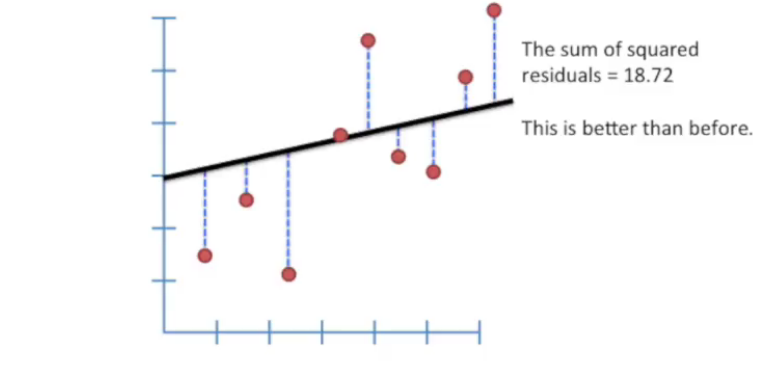
\includegraphics[width=0.8\linewidth,keepaspectratio]{statq60}
\end{center}

Its better but is this best?

\tiny{(Ref: StatQuest: Linear Models - Josh Starmer )}	

\end{frame}

%%%%%%%%%%%%%%%%%%%%%%%%%%%%%%%%%%%%%%%%%%%%%%%%%%%%%%%%%%%
\begin{frame}[fragile]\frametitle{Sum of Squared Errors for Rotated Line}
Rotated a bit more. Better?


\begin{center}
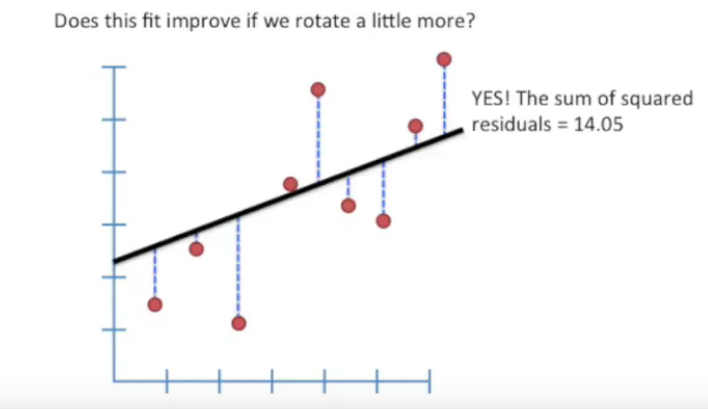
\includegraphics[width=0.8\linewidth,keepaspectratio]{statq61}
\end{center}

Its better but is this best?

\tiny{(Ref: StatQuest: Linear Models - Josh Starmer )}	

\end{frame}

%%%%%%%%%%%%%%%%%%%%%%%%%%%%%%%%%%%%%%%%%%%%%%%%%%%%%%%%%%%
\begin{frame}[fragile]\frametitle{Sum of Squared Errors for Rotated Line}
Why not rotate a whole lot!!


\begin{center}
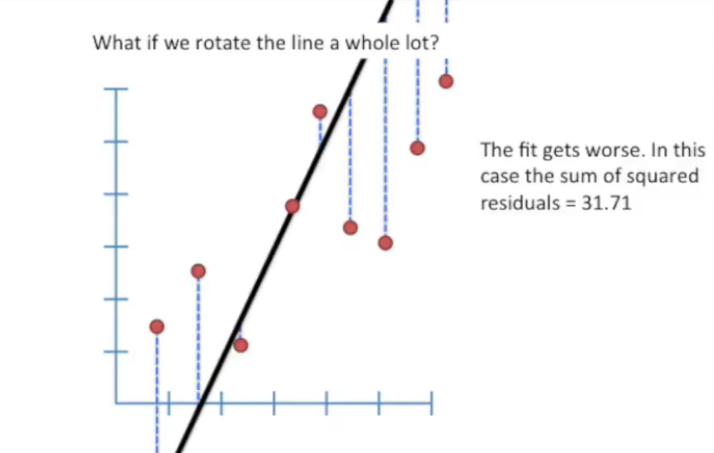
\includegraphics[width=0.7\linewidth,keepaspectratio]{statq62}
\end{center}

No, we lost the BEST point somewhere in between. Whats that ``optimized'' point?

\tiny{(Ref: StatQuest: Linear Models - Josh Starmer )}	

\end{frame}

%%%%%%%%%%%%%%%%%%%%%%%%%%%%%%%%%%%%%%%%%%%%%%%%%%%%%%%%%%%
\begin{frame}[fragile]\frametitle{Optimization}
To find the sweet spot ie the optimized point, lets put some formulation based on generic line equation.


\begin{center}
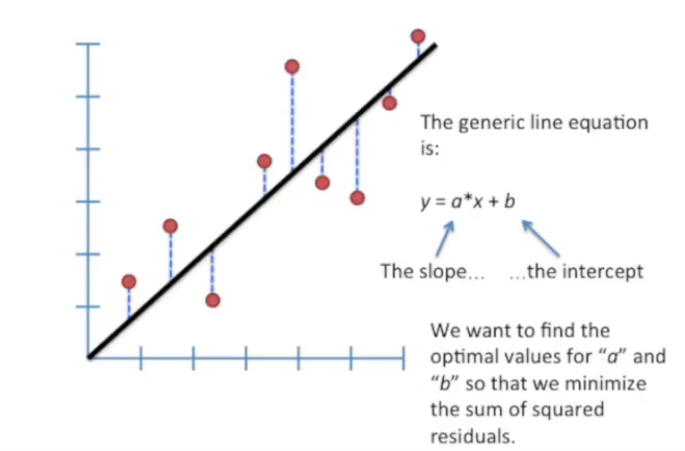
\includegraphics[width=0.7\linewidth,keepaspectratio]{statq63}
\end{center}



\tiny{(Ref: StatQuest: Linear Models - Josh Starmer )}	

\end{frame}

%%%%%%%%%%%%%%%%%%%%%%%%%%%%%%%%%%%%%%%%%%%%%%%%%%%%%%%%%%%
\begin{frame}[fragile]\frametitle{Optimization}
Mathematically \ldots

\begin{center}
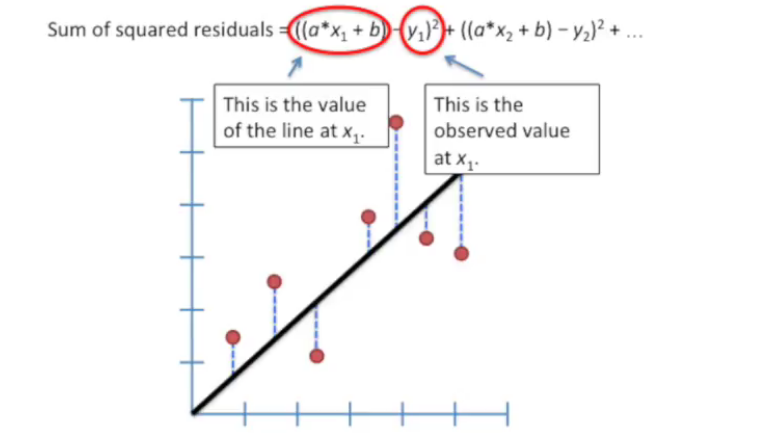
\includegraphics[width=0.7\linewidth,keepaspectratio]{statq64}
\end{center}

Since we want the line that will give us the smallest sum of the squares of errors (SSE: Sum of Squared Errors), this method for finding the best values for ``a'' and ``b'' is called as ``Least Squares''.

\tiny{(Ref: StatQuest: Linear Models - Josh Starmer )}	

\end{frame}

%%%%%%%%%%%%%%%%%%%%%%%%%%%%%%%%%%%%%%%%%%%%%%%%%%%%%%%%%%%
\begin{frame}[fragile]\frametitle{Optimization}
\begin{itemize}
\item If we plotted SSE for each rotated line the plot looks like. 
\item We can see that SSE was high for the horizontal line, then came down as we started rotating the line, 
\item But started rising again, if we passed the sweet spot.
\end{itemize}

\begin{center}
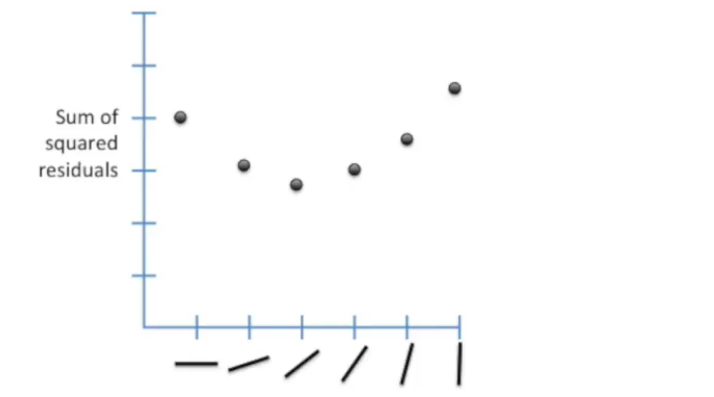
\includegraphics[width=0.7\linewidth,keepaspectratio]{statq65}
\end{center}

\tiny{(Ref: StatQuest: Linear Models - Josh Starmer )}	

\end{frame}

% %%%%%%%%%%%%%%%%%%%%%%%%%%%%%%%%%%%%%%%%%%%%%%%%%%%%%%%%%%%
% \begin{frame}[fragile]\frametitle{Optimization (Recap)}
% \begin{itemize}
% \item If we plotted SSE for each rotated line the plot looks like. 
% \item We can see that SSE was high for the horizontal line, then came down as we started rotating the line, 
% \item But started rising again, if we passed the sweet spot.
% \end{itemize}

% \begin{center}
% 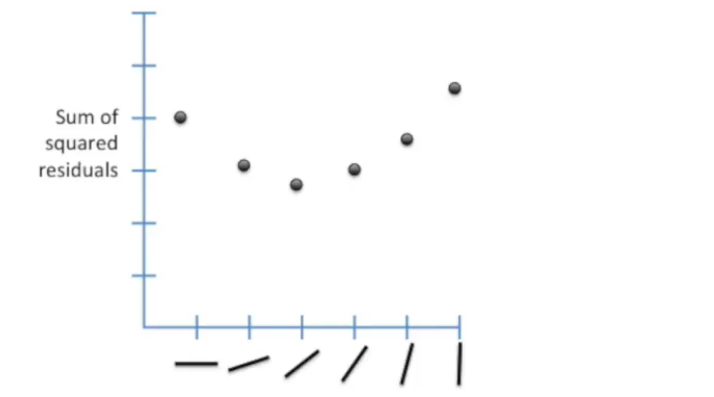
\includegraphics[width=0.8\linewidth,keepaspectratio]{statq65}
% \end{center}

% Whats the Machine Learning way of finding the Sweet Spot? Its Gradient Decent!!

% \tiny{(Ref: StatQuest: Linear Models - Josh Starmer )}	

% \end{frame}

%%%%%%%%%%%%%%%%%%%%%%%%%%%%%%%%%%%%%%%%%%%%%%%%%%%%%%%%%%%
\begin{frame}[fragile]\frametitle{Optimization}
\begin{itemize}
\item We need to get to the bottom point.
\item We can start at any (random) point, and SLIDE down to bottom.
\item SLIDING means going along slope. 
\item Slope is given by Derivative of the (SSE) function/curve, at the point 
\end{itemize}

\begin{center}
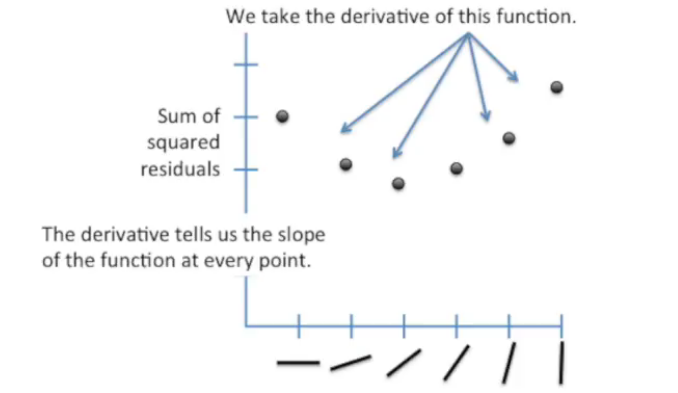
\includegraphics[width=0.7\linewidth,keepaspectratio]{statq66}
\end{center}

\tiny{(Ref: StatQuest: Linear Models - Josh Starmer )}	

\end{frame}

%%%%%%%%%%%%%%%%%%%%%%%%%%%%%%%%%%%%%%%%%%%%%%%%%%%%%%%%%%%
\begin{frame}[fragile]\frametitle{Optimization}
\begin{itemize}
\item Slope starts decreasing from end, faster,then slower,
\item Reaches 0, horizontal, and the starts increasing again.
\item Need to find the ``0'' slope point.
\end{itemize}

\begin{center}
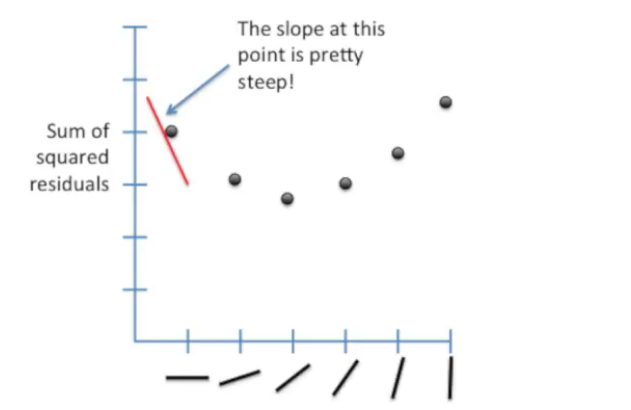
\includegraphics[width=0.24\linewidth,keepaspectratio]{statq67}
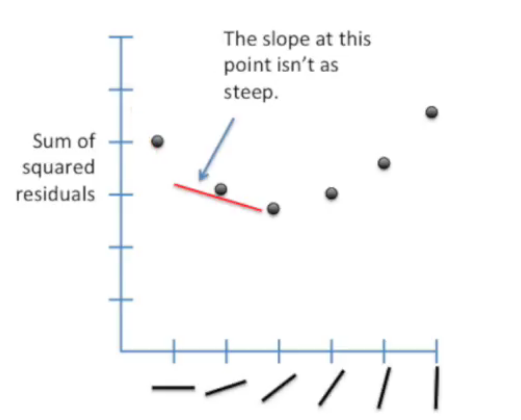
\includegraphics[width=0.24\linewidth,keepaspectratio]{statq68}
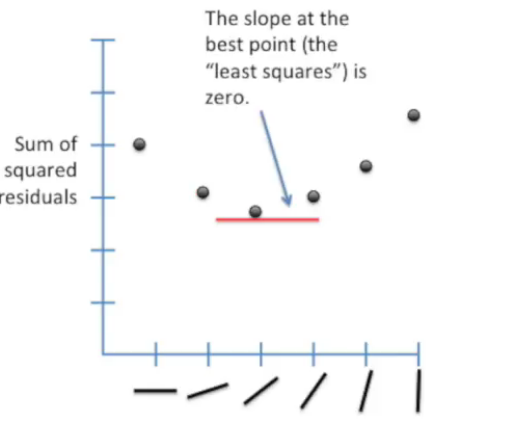
\includegraphics[width=0.24\linewidth,keepaspectratio]{statq69}
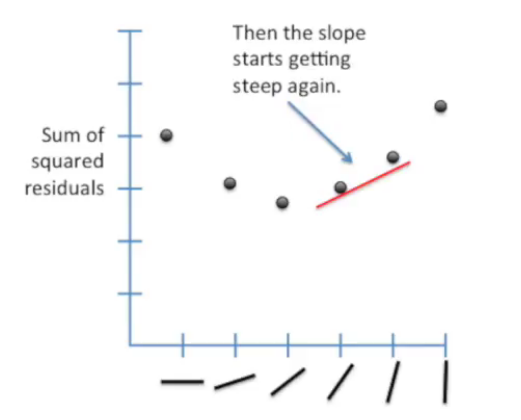
\includegraphics[width=0.24\linewidth,keepaspectratio]{statq70}
\end{center}

These different slopes means different ``a'' parameters
\tiny{(Ref: StatQuest: Linear Models - Josh Starmer )}	

\end{frame}


%%%%%%%%%%%%%%%%%%%%%%%%%%%%%%%%%%%%%%%%%%%%%%%%%%%%%%%%%%%
\begin{frame}[fragile]\frametitle{Optimization}

\begin{center}
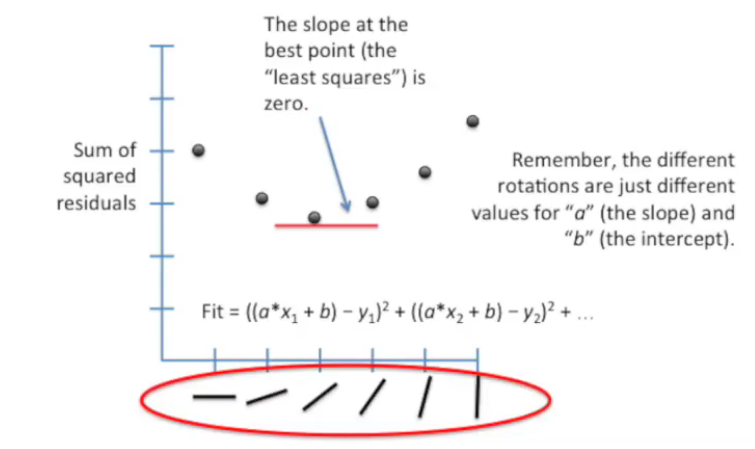
\includegraphics[width=0.7\linewidth,keepaspectratio]{statq71}
\end{center}

\tiny{(Ref: StatQuest: Linear Models - Josh Starmer )}	

\end{frame}


%%%%%%%%%%%%%%%%%%%%%%%%%%%%%%%%%%%%%%%%%%%%%%%%%%%%%%%%%%%
\begin{frame}[fragile]\frametitle{Optimization}
\begin{itemize}
\item For ``a'' and ``b'' both to be optimized, we will need 3D picture, as the Loss function would then take Z axis
\item It will be a Surface.
\item Derivative will be Partial, but the objective is the same, Bottom-most point. ie Minimum Loss function value
\end{itemize}

\begin{center}
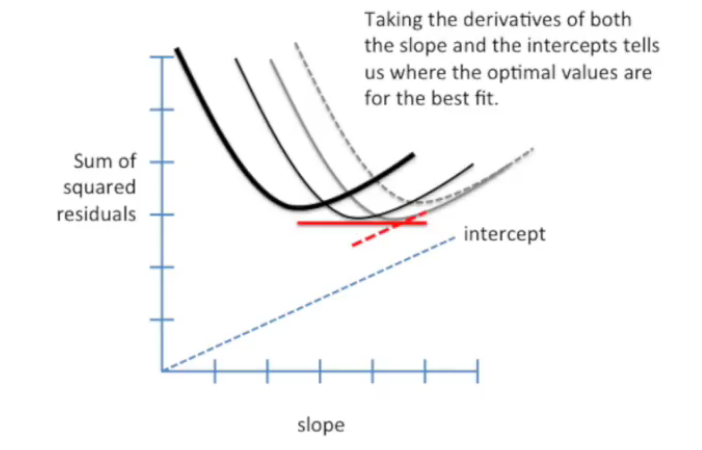
\includegraphics[width=0.5\linewidth,keepaspectratio]{statq72}
\end{center}

The '``a'' and ``b'' coordinates corresponding to the bottom-most point give most minimum Loss. So it represents the ``best'' line.

\tiny{(Ref: StatQuest: Linear Models - Josh Starmer )}	

\end{frame}

%%%%%%%%%%%%%%%%%%%%%%%%%%%%%%%%%%%%%%%%%%%%%%%%%%%%%%%%%%%
\begin{frame}[fragile]\frametitle{Results}

\begin{center}
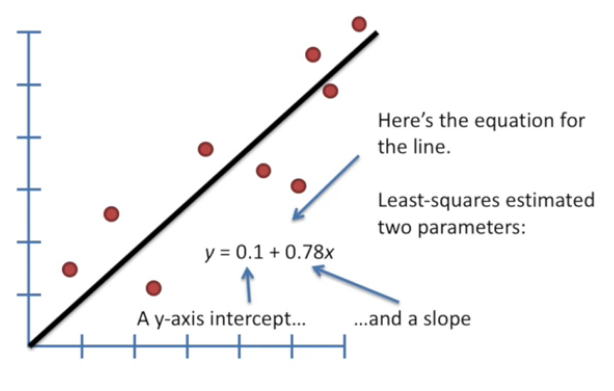
\includegraphics[width=0.7\linewidth,keepaspectratio]{statq73}
\end{center}

\tiny{(Ref: StatQuest: Linear Models - Josh Starmer )}	

\end{frame}


%%%%%%%%%%%%%%%%%%%%%%%%%%%%%%%%%%%%%%%%%%%%%%%%%%%%%%%%%%%
\begin{frame}[fragile]\frametitle{Example: Mouse Size }
\begin{itemize}
\item We have data points having mouse size and mouse weight
\item We wish to find mouse size given mouse weight.
\end{itemize}

\begin{center}
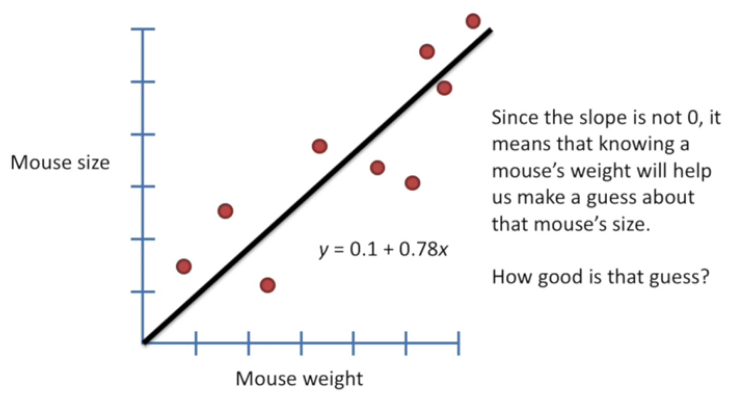
\includegraphics[width=0.7\linewidth,keepaspectratio]{statq74}
\end{center}

we use $R^2$ to find ``good-ness'' of fit (of line)

\tiny{(Ref: StatQuest: Linear Models - Josh Starmer )}	

\end{frame}



%%%%%%%%%%%%%%%%%%%%%%%%%%%%%%%%%%%%%%%%%%%%%%%%%%%%%%%%%%%%%%%%%%%%%%%%
\begin{frame}[fragile]\frametitle{Linear regression For Complex Problems}
\begin{itemize}
\item In real life, problems are far more complex that just one x and one y. 
\item There could be many x's ie many inputs which decide the output
\item General formulation : Predicting quantitative response $y$ based on predictor variables $x$. Assumes linear relationship between $x$ and $y$
\[
\begin{array}{rcl}
y_i &=& x_{1,i} \beta_1 + x_{2,i} \beta_2 + \cdots + x_{p,1} \beta_p + \epsilon_i
\end{array}
\]
\item Objective is to find the parameters $\beta_j$ that minimize the squared residuals 
\item There is no slope formulas for these $\beta$s. So, we will solve machine learning way.
\end{itemize}


\end{frame}



% %%%%%%%%%%%%%%%%%%%%%%%%%%%%%%%%%%%%%%%%%%%%%%%%%%%%%%%%%%%%%%%%%%%%%%%%%%%%%%%%%%
% \begin{frame}[fragile]\frametitle{}
% \begin{center}
% {\Large $R^2$ (Advance) }
% \end{center}
% \end{frame}


% %%%%%%%%%%%%%%%%%%%%%%%%%%%%%%%%%%%%%%%%%%%%%%%%%%%%%%%%%%%
% \begin{frame}[fragile]\frametitle{$R^2$ (Recap)}
% \begin{itemize}
% \item We take y values only. Take mean. Find diff with each y. Square and add. 
% \item We had called it SSE benchmark, but also called {\bf SS(mean)} is Sum of Squares around mean.
% \end{itemize}

% \begin{center}
% 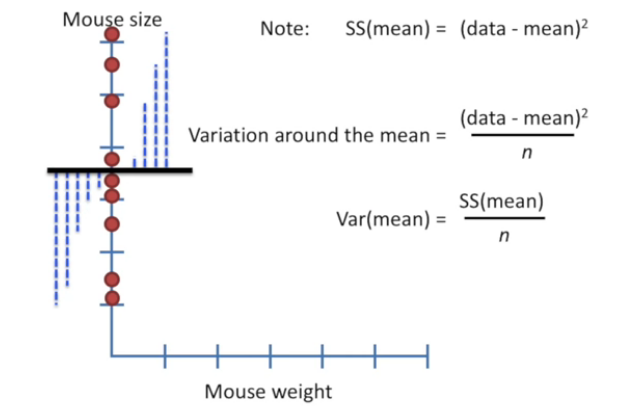
\includegraphics[width=0.8\linewidth,keepaspectratio]{statq75}
% \end{center}


% \tiny{(Ref: StatQuest: Linear Models - Josh Starmer )}	

% \end{frame}

% %%%%%%%%%%%%%%%%%%%%%%%%%%%%%%%%%%%%%%%%%%%%%%%%%%%%%%%%%%%
% \begin{frame}[fragile]\frametitle{$R^2$ (Recap)}

% Similarly {\bf SS(fit)} is Sum of Squares around the fitted line.

% \begin{center}
% 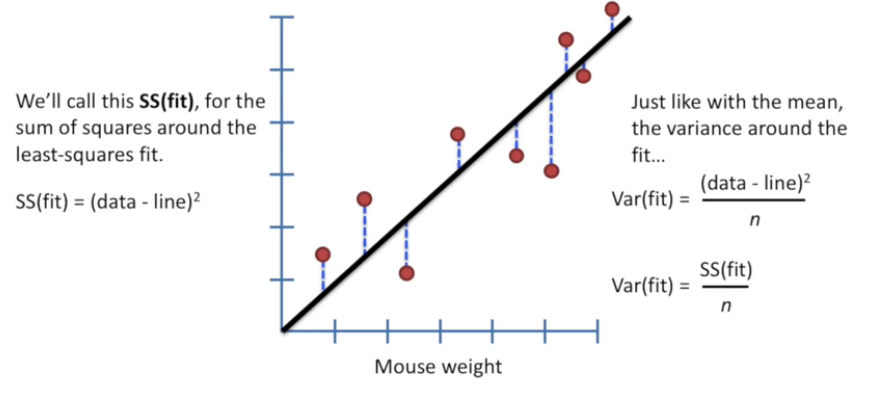
\includegraphics[width=0.8\linewidth,keepaspectratio]{statq76}
% \end{center}


% \tiny{(Ref: StatQuest: Linear Models - Josh Starmer )}	

% \end{frame}

% %%%%%%%%%%%%%%%%%%%%%%%%%%%%%%%%%%%%%%%%%%%%%%%%%%%%%%%%%%%
% \begin{frame}[fragile]\frametitle{$R^2$ (Recap)}

% Variations in fitted line (shown by blue dotted lines) is smaller.  So adding 'Weight' helps explain the variations.

% \begin{center}
% 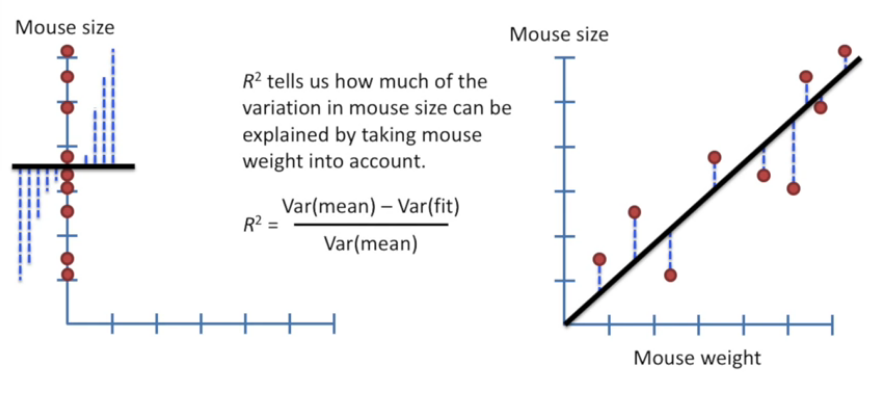
\includegraphics[width=0.8\linewidth,keepaspectratio]{statq77}
% \end{center}


% \tiny{(Ref: StatQuest: Linear Models - Josh Starmer )}	

% \end{frame}

% %%%%%%%%%%%%%%%%%%%%%%%%%%%%%%%%%%%%%%%%%%%%%%%%%%%%%%%%%%%
% \begin{frame}[fragile]\frametitle{$R^2$ (Recap)}

% Example:

% \begin{center}
% 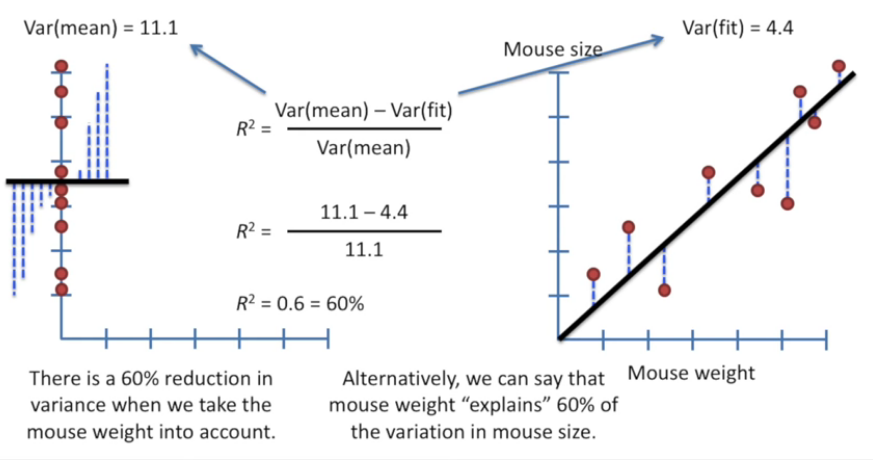
\includegraphics[width=0.8\linewidth,keepaspectratio]{statq78}
% \end{center}


% \tiny{(Ref: StatQuest: Linear Models - Josh Starmer )}	

% \end{frame}

% %%%%%%%%%%%%%%%%%%%%%%%%%%%%%%%%%%%%%%%%%%%%%%%%%%%%%%%%%%%
% \begin{frame}[fragile]\frametitle{Best $R^2$}

% Best $R^2$ is possible when there is no error in the fitted line. Meaning line passing through all points. But for that, data has to be collinear, else thats just not possible. Say, we have such lucky data, then \ldots

% \begin{center}
% 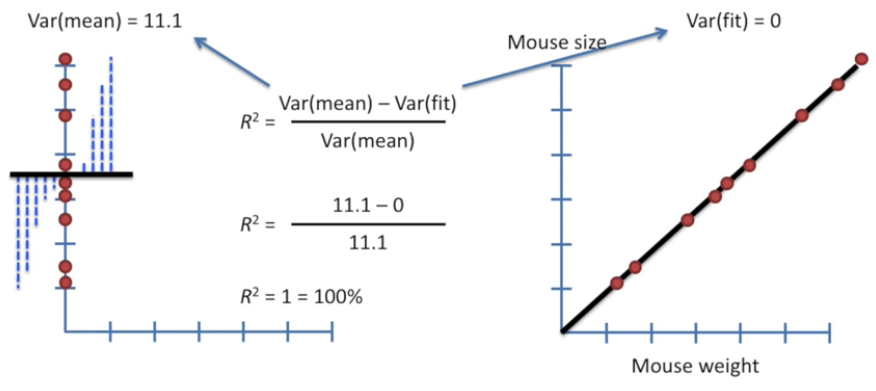
\includegraphics[width=0.8\linewidth,keepaspectratio]{statq79}
% \end{center}


% \tiny{(Ref: StatQuest: Linear Models - Josh Starmer )}	

% \end{frame}

% %%%%%%%%%%%%%%%%%%%%%%%%%%%%%%%%%%%%%%%%%%%%%%%%%%%%%%%%%%%
% \begin{frame}[fragile]\frametitle{Worst $R^2$}

% Worst $R^2$ is possible when there max errors in the fitted line. Thats the benchmark horizontal line.

% \begin{center}
% 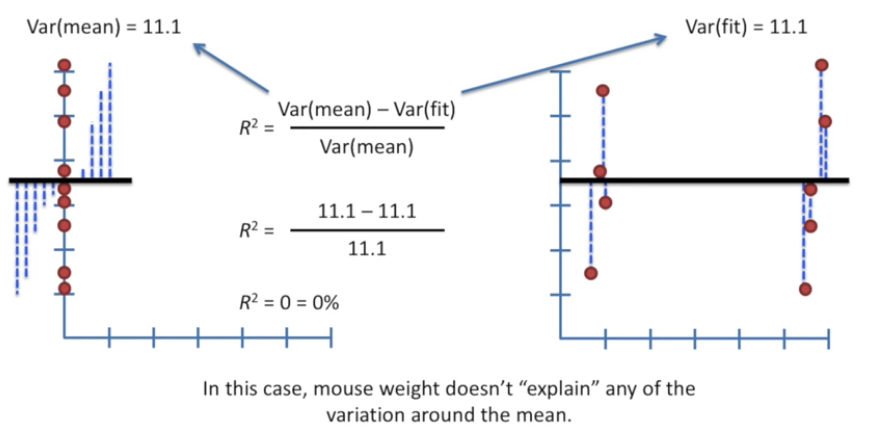
\includegraphics[width=0.8\linewidth,keepaspectratio]{statq80}
% \end{center}


% \tiny{(Ref: StatQuest: Linear Models - Josh Starmer )}	

% \end{frame}

% %%%%%%%%%%%%%%%%%%%%%%%%%%%%%%%%%%%%%%%%%%%%%%%%%%%%%%%%%%%
% \begin{frame}[fragile]\frametitle{Multivariate $R^2$}

% Even if you have a complicated equation with many x variables, the procedure is the same.

% \begin{center}
% 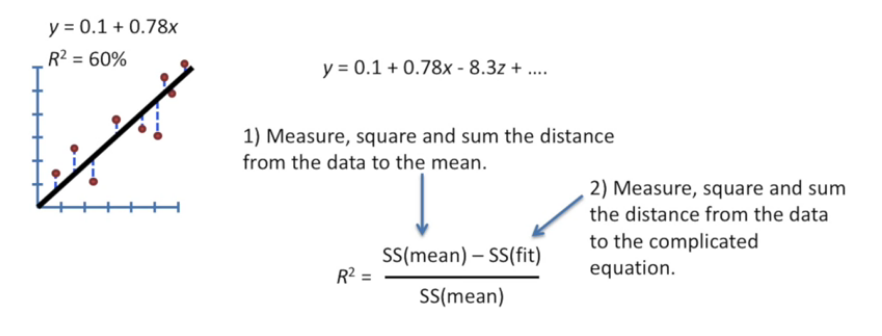
\includegraphics[width=\linewidth,keepaspectratio]{statq81}
% \end{center}


% \tiny{(Ref: StatQuest: Linear Models - Josh Starmer )}	

% \end{frame}

% %%%%%%%%%%%%%%%%%%%%%%%%%%%%%%%%%%%%%%%%%%%%%%%%%%%%%%%%%%%
% \begin{frame}[fragile]\frametitle{Multivariate $R^2$ Example}

% \begin{itemize}
% \item Output: Mouse Body Length
% \item Inputs : Mouse Weight (x) and Tail Length (z)
% \item Parameters to optimize: 3
% \end{itemize}

% Using Gradient Decent we got those \ldots

% \begin{center}
% 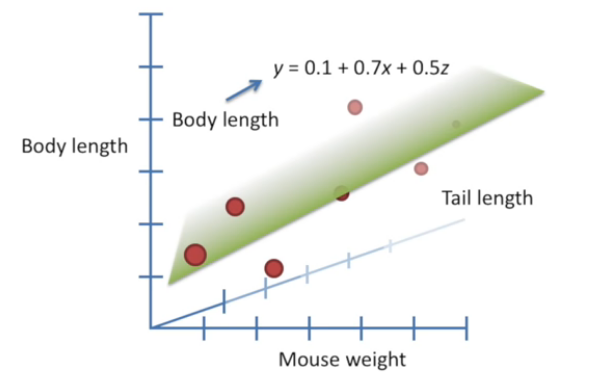
\includegraphics[width=0.6\linewidth,keepaspectratio]{statq82}
% \end{center}

% The model is plane (not a 3D line)

% \tiny{(Ref: StatQuest: Linear Models - Josh Starmer )}	

% \end{frame}

% %%%%%%%%%%%%%%%%%%%%%%%%%%%%%%%%%%%%%%%%%%%%%%%%%%%%%%%%%%%
% \begin{frame}[fragile]\frametitle{Many variables }

% If it turns out that the weight for tail length is minimum (or zero). So no effect.

% \begin{center}
% 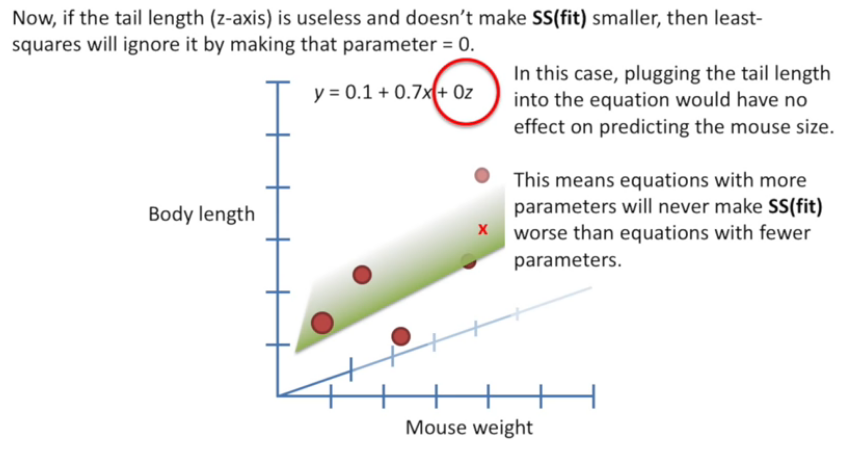
\includegraphics[width=0.8\linewidth,keepaspectratio]{statq83}
% \end{center}

% \tiny{(Ref: StatQuest: Linear Models - Josh Starmer )}	

% \end{frame}

% %%%%%%%%%%%%%%%%%%%%%%%%%%%%%%%%%%%%%%%%%%%%%%%%%%%%%%%%%%%
% \begin{frame}[fragile]\frametitle{Adjusted $R^2$}

% \begin{itemize}
% \item More useless features we add, we get more variables for optimization to play with. 
% \item But these  (by chance) may improve $R^2$. Thats Bad!!
% \item We need ``adjusted $R^2$'' value that scales $R^2$ by the number of parameters.
% \end{itemize}

% \begin{center}
% 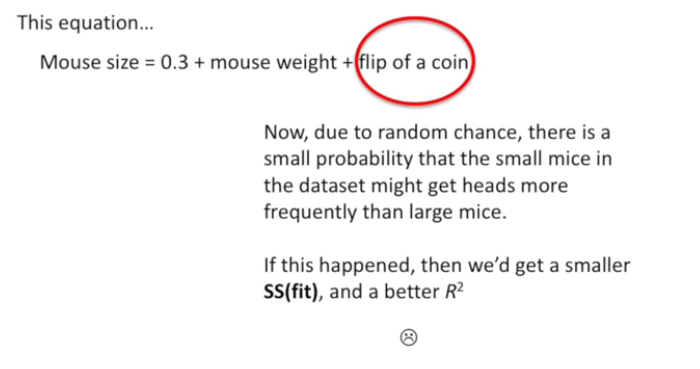
\includegraphics[width=0.6\linewidth,keepaspectratio]{statq84}
% \end{center}


% \tiny{(Ref: StatQuest: Linear Models - Josh Starmer )}	

% \end{frame}

% %%%%%%%%%%%%%%%%%%%%%%%%%%%%%%%%%%%%%%%%%%%%%%%%%%%%%%%%%%%
% \begin{frame}[fragile]\frametitle{Limitations of $R^2$}


% \begin{itemize}
% \item Say, we have only 2 points. {\bf SS(mean) = 10} and {\bf SS(fit)} will always be 0 as the line will pass through these two points.
% \item Here, $R^2$ is 1. So any two points in data set has same $R^2 = 1$.
% \item Need to find if the $R^2$ that we have for the fitted line, is it statistically significant.
% \item Thats done by p-value.
% \end{itemize}


% \tiny{(Ref: StatQuest: Linear Models - Josh Starmer )}	

% \end{frame}

% %%%%%%%%%%%%%%%%%%%%%%%%%%%%%%%%%%%%%%%%%%%%%%%%%%%%%%%%%%%
% \begin{frame}[fragile]\frametitle{p-value of $R^2$}
% \begin{itemize}
% \item p-value for $R^2$ comes from something called ``F''.
% \item Its a ratio of The variation in y explained by one x, divided by the variation in y NOT explained by that x
% \end{itemize}

% \begin{center}
% 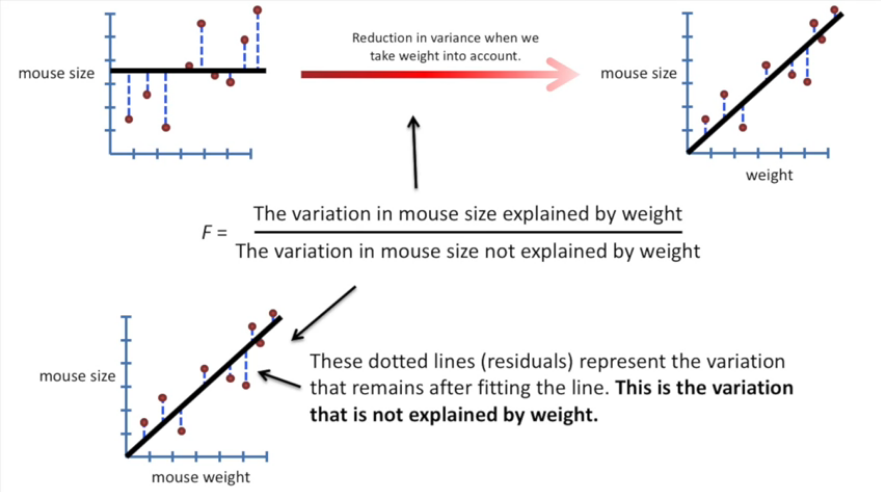
\includegraphics[width=0.8\linewidth,keepaspectratio]{statq85}
% \end{center}

% \tiny{(Ref: StatQuest: Linear Models - Josh Starmer )}	

% \end{frame}

% %%%%%%%%%%%%%%%%%%%%%%%%%%%%%%%%%%%%%%%%%%%%%%%%%%%%%%%%%%%
% \begin{frame}[fragile]\frametitle{p-value of $R^2$}
% \begin{itemize}
% \item Terms in denominators are degrees of freedom.
% \item $p_{fit}$ : number of parameters in fit line: 2: slope and intercept
% \item $p_{mean}$ : number of parameters in mean-benchmark line: 1: only intercept
% \item The whole numerator is variations explained by features ie mouse weight.
% \item The whole numerator is variations NOT explained by features.
% \item Why divide by $n - p_{fir}$ instead of just $n$?: Intuitively, the more features, more data needed to estimate them.
% \item If the fit (``F'') is good, we have large number in numerator (most variance got explained) and smaller number in denominator. That make ``F'' very large number. How to convert this to a p-value?
% \end{itemize}

% \begin{center}
% 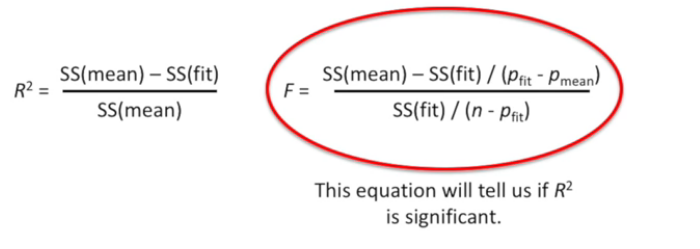
\includegraphics[width=0.6\linewidth,keepaspectratio]{statq86}
% \end{center}

% \tiny{(Ref: StatQuest: Linear Models - Josh Starmer )}	

% \end{frame}

% %%%%%%%%%%%%%%%%%%%%%%%%%%%%%%%%%%%%%%%%%%%%%%%%%%%%%%%%%%%
% \begin{frame}[fragile]\frametitle{p-value of $R^2$}
% \begin{itemize}
% \item Generate many random datasets.
% \item Find Fs for all of them.
% \item Plot the histogram. We get the distribution
% \item Is our F, on the tail side of this distribution? Thats found by p-value.
% \end{itemize}

% \begin{center}
% 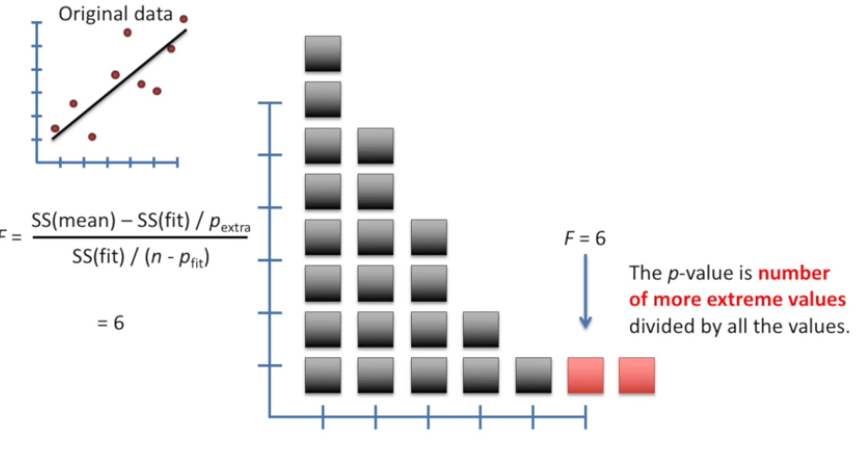
\includegraphics[width=0.6\linewidth,keepaspectratio]{statq87}
% \end{center}

% \tiny{(Ref: StatQuest: Linear Models - Josh Starmer )}	

% \end{frame}


% %%%%%%%%%%%%%%%%%%%%%%%%%%%%%%%%%%%%%%%%%%%%%%%%%%%%%%%%%%%
% \begin{frame}[fragile]\frametitle{p-value of $R^2$}
% \begin{itemize}
% \item Standard F distributions are available for different degrees of freedom.
% \item Calculate p value for your F
% \end{itemize}

% \begin{center}
% 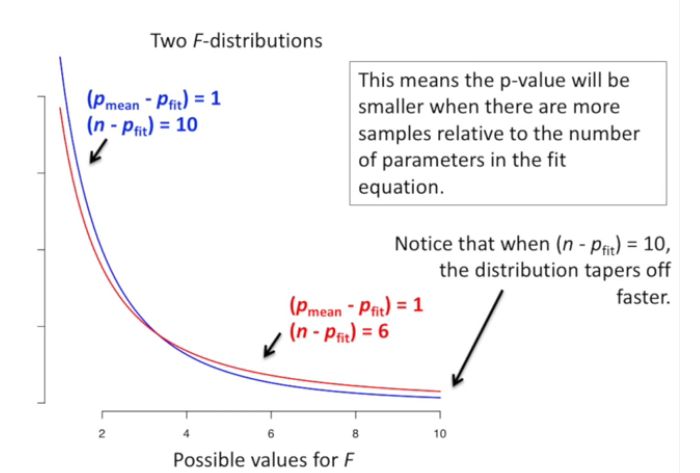
\includegraphics[width=0.6\linewidth,keepaspectratio]{statq88}
% \end{center}

% Need $R^2$ to be large and p-value to be small, so has to have a good fit line.

% \tiny{(Ref: StatQuest: Linear Models - Josh Starmer )}	

% \end{frame}

% %%%%%%%%%%%%%%%%%%%%%%%%%%%%%%%%%%%%%%%%%%%%%%%%%%%%%%%%%%%
% \begin{frame}[fragile]\frametitle{Linear regression Objective}
% \begin{center}
% 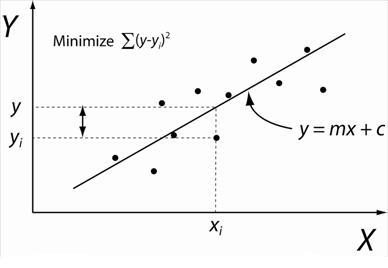
\includegraphics[width=0.8\linewidth,keepaspectratio]{linreg}
% \end{center}
% \end{frame}

%%%%%%%%%%%%%%%%%%%%%%%%%%%%%%%%%%%%%%%%%%%%%%%%%%%%%%%%%%%%
%\begin{frame}[fragile]\frametitle{Linear regression}
%\begin{lstlisting}
%import numpy as np
%import matplotlib.pyplot as plt
%
%# Random data
%N = 10
%M = 2
%input = np.random.random((N,M))
%print input 
%
%# Setup matrices
%m = np.shape(input)[0]
%X = np.matrix([np.ones(m), input[:,0]]).T
%y = np.matrix(input[:,1]).T
%
%# Solve for projection matrix
%p_mat = np.linalg.inv(X.T.dot(X)).dot(X.T).dot(y)
%print p_mat
%
%# Find regression line
%xx = np.linspace(0, 1, 2)
%yy = np.array(p_mat[0] + p_mat[1] * xx)
%\end{lstlisting}
%\end{frame}
%
%%%%%%%%%%%%%%%%%%%%%%%%%%%%%%%%%%%%%%%%%%%%%%%%%%%%%%%%%%%%
%\begin{frame}[fragile]\frametitle{Linear regression}
%%A particular run of this code generates the following input matrix:
%%\begin{lstlisting}
%%[[ 0.64840322  0.97285346]
%% [ 0.77867147  0.87310339]
%% [ 0.85072744  0.59023482]
%% [ 0.3692784   0.59567815]
%% [ 0.14654649  0.79422356]
%% [ 0.46897942  0.06988269]
%% [ 0.79239438  0.33157126]
%% [ 0.88935174  0.04946074]
%% [ 0.0615097   0.68082408]
%% [ 0.63675227  0.93102028]]
%%\end{lstlisting}
%The values of which are the y-intercept and slope of the regression line, respectively:
%\begin{lstlisting}
%[[ 0.73461589]
% [-0.25826794]]
%\end{lstlisting}
%\begin{center}
%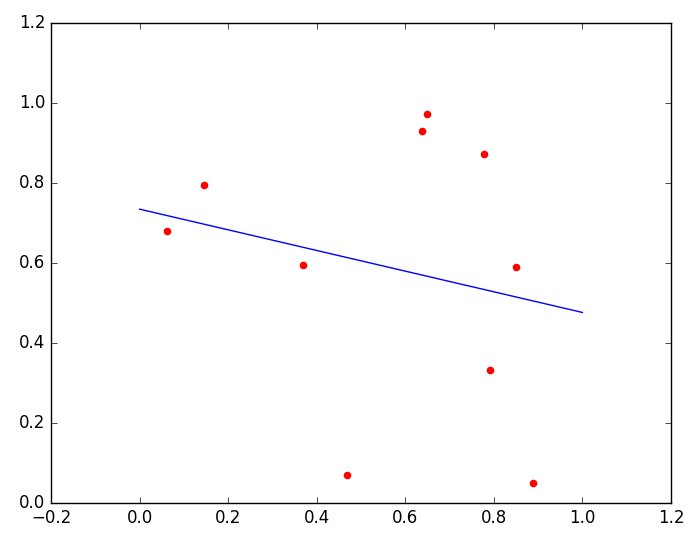
\includegraphics[width=0.6\linewidth,keepaspectratio]{linreg2}
%\end{center}
%\end{frame}




% %%%%%%%%%%%%%%%%%%%%%%%%%%%%%%%%%%%%%%%%%%%%%%%%%%%
% \begin{frame}[fragile]\frametitle{Constants}
% In one dimensional case:
% \[
% \begin{array}{rcl}
% y_i &=& \beta_0 + x_i \beta_1 + \epsilon_i
% \end{array}
% \]
% $\beta_0$ is intercept and $\beta_1$ is the slope of the line.
% \end{frame}

% %%%%%%%%%%%%%%%%%%%%%%%%%%%%%%%%%%%%%%%%%%%%%%%%%%%
% \begin{frame}[fragile]\frametitle{Constants}
% Use training data to produce estimates for the model coefficients.
% \begin{center}
% 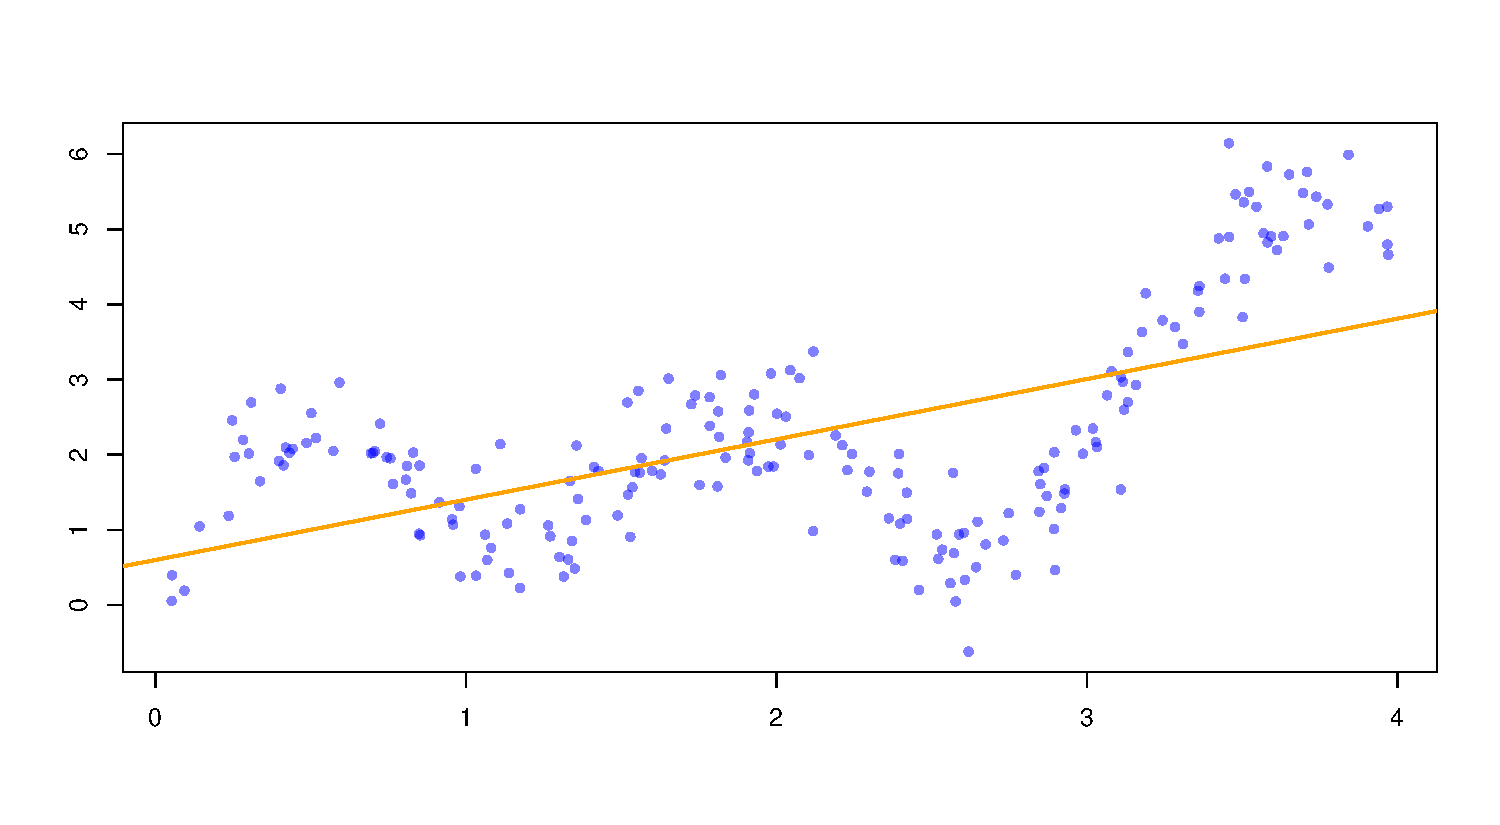
\includegraphics[width=0.8\linewidth]{olsSimple.pdf}
% \end{center}
% \end{frame}


% %%%%%%%%%%%%%%%%%%%%%%%%%%%%%%%%%%%%%%%%%%%%%%%%%%%%%%%%%%%%%%%%%%%%%%%%
% \begin{frame}[fragile]\frametitle{Estimating the Coefficients}
% \begin{itemize}
% \item Goal is to obtain coefficient estimates such that the linear model fits the available data well
	% \begin{itemize}
	% \item To find an intercept $\beta_0$ and slope $\beta_1$ such that the resulting line is as close as possible to the data points
	% \item Q: How to determine ``closeness''? Whats the Error/Cost entity to be minimized?
	% \item A: Common approach: least squares
	% \end{itemize}
% \end{itemize}
% %\begin{center}
% %\includegraphics[width=0.6\linewidth]{regr}
% %\end{center}
% \end{frame}

% %%%%%%%%%%%%%%%%%%%%%%%%%%%%%%%%%%%%%%%%%%%%%%%%%%%%%%%%%%%%%%%%%%%%%%%%
% \begin{frame}[fragile]\frametitle{Residual Sum of Squares (RSS)}
% \begin{itemize}
% \item Prediction for $y$ based on the $i^{th}$ value of $x$
% \[
% \begin{array}{c}
% \hat{y_i} = \hat{\beta_0} + x_i \hat{\beta_1}
% \end{array}
% \]
% \item $i^{th}$ : residual: difference between the $i^{th}$ observed response value and the $i^{th}$ predicted value
% \[
% \begin{array}{c}
% e_i= y_i - \hat{y_i}
% \end{array}
% \]
% \item Residual Sum of Squares (RSS):
% \[
% \begin{array}{c}
% RSS= e_1^2 + e_2^2 + e_3^2 + \ldots
% \end{array}
% \]
% \end{itemize}
% Least Squares: chooses $\hat{\beta_0}$ and $\hat{\beta_1}$   to minimize the RSS

% \end{frame}


% %%%%%%%%%%%%%%%%%%%%%%%%%%%%%%%%%%%%%%%%%%%%%%%%%%%%%%%%%%%
% \begin{frame}[fragile]\frametitle{Why Squared error?}
	% \begin{itemize}
	% \item  Why we choose to minimize the mean square error instead of something else? After all, one can minimize the mean absolute value of the residual. 
	% \item Reason: There is no good minima to absolute value (ie Linear) function. Its actually at infinity, which is of no use.
	% \item But Squared Error function may have cusp, so a good minima value.
	% \end{itemize}
	
% \end{frame}

% %%%%%%%%%%%%%%%%%%%%%%%%%%%%%%%%%%%%%%%%%%%%%%%%%%%%%%%%%%%
% \begin{frame}[fragile]\frametitle{Why Squared error?}
% \begin{center}
% \includegraphics[width=0.8\linewidth,keepaspectratio]{shil1}
% \end{center}	
% {\tiny (Ref: Introduction to Machine Learning - Shiladitya}
% \end{frame}



% %%%%%%%%%%%%%%%%%%%%%%%%%%%%%%%%%%%%%%%%%%%%%%%%%%%%%%%%%%%%%%%%%%%%%%%
% \begin{frame}[fragile]\frametitle{Least Squares}
% Using some Calculus, can show:
% \begin{center}
% \includegraphics[width=0.4\linewidth]{rss}
% \end{center}
% \end{frame}

% %%%%%%%%%%%%%%%%%%%%%%%%%%%%%%%%%%%%%%%%%%%%%%%%%%%%%%%%%%%%%%%%%%%%%%%%%%%%%%%%%%
% \begin{frame}[fragile]\frametitle{}
% \begin{center}
% {\Large Linear Regression - Car Purchase Example}
% \end{center}
% \end{frame}


% %%%%%%%%%%%%%%%%%%%%%%%%%%%%%%%%%%%%%%%%%%%%%%%%%%%%%%%%%%%%%%%%%%%%%%%%
% \begin{frame}[fragile]\frametitle{Example}
% \begin{itemize}
% \item  You wish to buy a car
% \item You find out car characteristics and their respective prices for some of the cars from a dealer friend
% \end{itemize}
% \begin{center}
% \includegraphics[width=0.5\linewidth]{carex1}
% \end{center}
% \end{frame}

% %%%%%%%%%%%%%%%%%%%%%%%%%%%%%%%%%%%%%%%%%%%%%%%%%%%%%%%%%%%%%%%%%%%%%%%%
% \begin{frame}[fragile]\frametitle{Questions}
% Want to evaluate if indeed one can predict car price based on engine size. The first set of analysis seeks the answers to the following questions:
% \begin{itemize}
% \item Is price of car related with engine size?
% \item How strong is the relationship?
% \item Is the relationship linear?
% \item Can we predict/estimate car price based on engine size?
% \end{itemize}
% \end{frame}

% %%%%%%%%%%%%%%%%%%%%%%%%%%%%%%%%%%%%%%%%%%%%%%%%%%%%%%%%%%%%%%%%%%%%%%%
% \begin{frame}[fragile]\frametitle{Theoretically}
% H0 and Ha need to be defined. They are defined as follows:
% \begin{itemize}
% \item H0 (NULL hypothesis): There is no relationship between x and y i.e. between price and engine size.
% \item Ha (Alternate hypothesis): There is some relationship between x and y.
% \item We can safely reject the NULL hypothesis and accept the alternate hypothesis if there is a robust relationship between price and engine size
% \end{itemize}
% \end{frame}

% %%%%%%%%%%%%%%%%%%%%%%%%%%%%%%%%%%%%%%%%%%%%%%%%%%%%%%%%%%%%%%%%%%%%%%%%
% \begin{frame}[fragile]\frametitle{Exploratory Data Analysis}
% \begin{itemize}
% \item You do a correlation analysis. Correlation is a measure of how much the two variables are related.
% \item It is measured by a metric called as the correlation coefficient. Its value is between 0 and 1.
% \item Plot the relationship between price and engine size.
% \end{itemize}
% \end{frame}


% %%%%%%%%%%%%%%%%%%%%%%%%%%%%%%%%%%%%%%%%%%%%%%%%%%%%%%%%%%%%%%%%%%%%%%%%
% \begin{frame}[fragile]\frametitle{Exploratory Data Analysis}
% \begin{center}
% \includegraphics[width=0.8\linewidth]{carex2}
% \end{center}
% Build a linear regression model that will estimate the price of the car price based on engine size.
% \end{frame}

% %%%%%%%%%%%%%%%%%%%%%%%%%%%%%%%%%%%%%%%%%%%%%%%%%%%%%%%%%%%%%%%%%%%%%%%%
% \begin{frame}[fragile]\frametitle{Model}
% $price = -6870.1 + 156.9 \times EngineSize$
% \begin{center}
% \includegraphics[width=0.65\linewidth]{carex3}
% \end{center}
% \end{frame}

% %%%%%%%%%%%%%%%%%%%%%%%%%%%%%%%%%%%%%%%%%%%%%%%%%%%%%%%%%%%%%%%%%%%%%%%%
% \begin{frame}[fragile]\frametitle{Testing and Prediction}
% \begin{center}
% \includegraphics[width=0.7\linewidth]{carex4}
% \end{center}
% \end{frame}


%%%%%%%%%%%%%%%%%%%%%%%%%%%%%%%%%%%%%%%%%%%%%%%%%%%%%%%%%%%%%%%%%%%%%%%%%%%%%%%%%%
\begin{frame}[fragile]\frametitle{}
\begin{center}
{\Large Linear Regression - Advertising Budget Example}
\end{center}
\end{frame}

%%%%%%%%%%%%%%%%%%%%%%%%%%%%%%%%%%%%%%%%%%%%%%%%%%%%%%%%%%%%%%%%%%%%%%%%
\begin{frame}[fragile]\frametitle{Example: Advertising Dataset}
\begin{itemize}
\item Toy Dataset: Advertising, Advertising.csv 
\item Sales totals for a product in 200 different markets. Advertising budget in each market, broken down into TV, radio, newspaper
\end{itemize}
%\begin{lstlisting}
%import pandas as pd
%advertising = pd.read_csv('../datasets/Advertising.csv')
%advertising.head(5)
%\end{lstlisting}
\begin{center}
\includegraphics[width=0.8\linewidth]{advtdata}
\end{center}
({\small Data: http://www-bcf.usc.edu/\~ gareth/ISL/data.html)}
\end{frame}


%%%%%%%%%%%%%%%%%%%%%%%%%%%%%%%%%%%%%%%%%%%%%%%%%%%%%%%%%%%%%%%%%%%%%%%%
\begin{frame}[fragile]\frametitle{Problem}
\begin{itemize}
\item Goal: What marketing plan for next year will result in high product sales?
\item Questions (Hypothesis):
	\begin{itemize}
	\item Is there a relationship between advertising budgets and sales?
	\item How strong is the relationship between advertising budgets and sales?
	\item Which media contribute to the sales the most?
%	\item How accurately can we estimate the effect of each medium on sales?
	\item Is the relationship linear?
%	\item Is there any interaction effect? (called ``synergy'' in business). Example: spending 50k on TV ads + 50k on radio ads results in more sales than spending 100k on only TV
	\end{itemize}
\end{itemize}
\end{frame}


%%%%%%%%%%%%%%%%%%%%%%%%%%%%%%%%%%%%%%%%%%%%%%%%%%%%%%%%%%%%%%%%%%%%%%%%
\begin{frame}[fragile]\frametitle{EDA}
Correlation Matrix

\begin{center}
\includegraphics[width=0.8\linewidth]{corrmat}
\end{center}
\begin{itemize}
\item Correlation between radio and newspaper is 0.35
\item Barely any correlation (or ``not correlated'') for TV/radio and TV/newspaper
\end{itemize}
\end{frame}

%%%%%%%%%%%%%%%%%%%%%%%%%%%%%%%%%%%%%%%%%%%%%%%%%%%%%%%%%%%%%%%%%%%%%%%%
\begin{frame}[fragile]\frametitle{EDA}
\begin{center}
\includegraphics[width=0.8\linewidth]{corrmat}
\end{center}
\begin{itemize}
\item Reveals tendency to spend more on Newspaper advertising in markets where more is spent on Radio advertising.
\item Sales higher in markets where more is spent on Radio, but more also tends to be spent on Newspaper.
\item In Simple LM: Newspaper ``gets credit'' for effect of Radio on Sales.
\end{itemize}
\end{frame}
%%%%%%%%%%%%%%%%%%%%%%%%%%%%%%%%%%%%%%%%%%%%%%%%%%%%%%%%%%%%%%%%%%%%%%%%
\begin{frame}[fragile]\frametitle{Advertising Dataset}
\begin{itemize}
\item What are some ways we can regress sales onto adverting using Simple Linear Regression?
\item One model:

\begin{eqnarray*}
sales & \approx \beta_0 +  \beta_1 \times TV \\
y & \approx \beta_0 + \beta_1 \times x
\end{eqnarray*}

\item Scatter plot visualization for TV and Sales.
%\begin{lstlisting}
%%matplotlib inline
%advertising.plot.scatter(x='TV', y='Sales');
%\end{lstlisting}
\begin{center}
\includegraphics[width=0.4\linewidth]{advtscatter}
\end{center}
\end{itemize}
\end{frame}

%%%%%%%%%%%%%%%%%%%%%%%%%%%%%%%%%%%%%%%%%%%%%%%%%%%%%%%%%%%%%%%%%%%%%%%%
\begin{frame}[fragile]\frametitle{Advertising Dataset}
\begin{itemize}
\item Simple Linear Model in Python (using pandas and scikit): Predictor: $x$, Response: $y$
%\begin{lstlisting}
%reg = linear_model.LinearRegression()
%reg.fit(advertising['TV'].reshape(-1,1), advertising['Sales'].reshape(-1,1))
%print('Coefficients: \n', reg.coef_)
%print('Intercept: \n', reg.intercept_)
%
%Coefficients: [[ 0.04753664]] 
%Intercept: [ 7.03259355]
%\end{lstlisting}
\item $Sales = 7.03259 + 0.04754  \times  TV$
\end{itemize}
\end{frame}

%%%%%%%%%%%%%%%%%%%%%%%%%%%%%%%%%%%%%%%%%%%%%%%%%%%%%%%%%%%%%%%%%%%%%%%%
\begin{frame}[fragile]\frametitle{Advertising Dataset}
Scatter plot visualization for TV and Sales with Linear Model.
%\begin{lstlisting}
%plt.scatter(advertising['TV'], advertising['Sales'],  color='black')
%plt.plot(advertising['TV'], reg.predict(advertising['TV'].reshape(-1,1)), 
%         color='blue', linewidth=3)
%
%\end{lstlisting}
\begin{center}
\includegraphics[width=0.6\linewidth]{advtscatterline}
\end{center}

If we have 3 such models, can we ``somehow'' compose them (say, averaging) to get the combined model?

\end{frame}

%
%%%%%%%%%%%%%%%%%%%%%%%%%%%%%%%%%%%%%%%%%%%%%%%%%%%%%%%%%%%%%%%%%%%%%%%%%
%\begin{frame}[fragile]\frametitle{Quality}
%Measuring the Quality of a Regression Model. Residual Standard Error
%\begin{array}
%RSE = \sqrt{\frac{RSS}{(n-2)}}
%\end{array}
%Advertising Dataset
%$RSE = 3.2586563 \approx 3.25$
%Confidence Interval for the Mean Value of $y$ given $x$
%\begin{center}
%\includegraphics[width=0.4\linewidth]{advtconf}
%\end{center}
%\end{frame}
%
%
%%%%%%%%%%%%%%%%%%%%%%%%%%%%%%%%%%%%%%%%%%%%%%%%%%%%%%%%%%%%%%%%%%%%%%%%%
%\begin{frame}[fragile]\frametitle{Comparison: Confidence Interval vs. Prediction Interval}
%Analogy
%\begin{itemize}
%\item Trying to predict baseball batting average
%\item ``Team'' batting averages (mean of the player batting averages on that team), for all 30 teams, have low variance. Should be easier to predict a team batting average
%\item ``Individual batting averages are quite varied (some players are good, while some players are Ryan Howard). Estimate of team average will be more precise than an estimate of a randomly chosen player, for the same level of confidence
%\end{itemize}
%\end{frame}
%
%%%%%%%%%%%%%%%%%%%%%%%%%%%%%%%%%%%%%%%%%%%%%%%%%%%%%%%%%%%%%%%%%%%%%%%%%
%\begin{frame}[fragile]\frametitle{Evaluating using a Test Set}
%%Given a set of predictions for m new cases, we can evaluate the model's predictions by
%\begin{itemize}
%\item Mean Error (ME): should be close to zero
%\begin{center}
%\includegraphics[width=0.4\linewidth]{meanerr}
%\end{center}
%%\item Residual Standard Error:$RSE = \sqrt{\frac{RSS}{(n-2)}}$
%\item Root Mean Square Error (RMSE)
%\begin{center}
%\includegraphics[width=0.4\linewidth]{meanrsqr}
%\end{center}
%%\item Mean Absolute Percent Error (MAPE)
%%\begin{center}
%%\includegraphics[width=0.4\linewidth]{meanmape}
%%\end{center}
%\end{itemize}
%\end{frame}

%%%%%%%%%%%%%%%%%%%%%%%%%%%%%%%%%%%%%%%%%%%%%%%%%%%%%%%%%%%%%%%%%%%%%%%%%%
%%\begin{frame}[fragile]\frametitle{Advertising Dataset}
%%\begin{itemize}
%%\item RSE = 3.26. Actual sales in each market deviate from the true regression line by approximately 3.26 units, on average.
%%\item Is this error amount acceptable?
%%\item Business answer: depends on problem context
%%\item Worth noting the percentage error:
%%$PercentageError = \frac{RSE}{Mean\_Sales} = \frac{3.26}{14} = 0.23238 = 23\%$
%%\item RSE measures the ``lack of fit'' that a model may have.
%%
%%\end{itemize}
%%\end{frame}





%%%%%%%%%%%%%%%%%%%%%%%%%%%%%%%%%%%%%%%%%%%%%%%%%%%%%%%%%%%%%%%%%%%%%%%%
\begin{frame}[fragile]\frametitle{Multiple Linear Regression}
\begin{itemize}
\item In practice, often have more than one predictor
\begin{itemize}
\item $sales \approx \beta_{0,1} + \beta_{1,1} \times TV$
\item $sales \approx \beta_{0,2} + \beta_{1,2} \times Newspaper$
\item $sales \approx \beta_{0,3} + \beta_{1,3} \times radio$
\end{itemize}
\item Run three separate simple linear regressions
\item For p predictor variables:
$ Y = \beta_0 + \beta_1 X_1 + \beta_2 X_2 + \ldots + \beta_p X_p + \epsilon$
\item Since error $\epsilon$ has mean zero, we usually omit it.
\item A one-unit change in any predictor variable $x_i$ will change the expected mean response by $\beta_j$ units. 
$ sales = \beta_0 + \beta_1 \times TV + \beta_2 \times radio + \beta_3 \times newspaper$
\end{itemize}
\end{frame}


%%
%%%%%%%%%%%%%%%%%%%%%%%%%%%%%%%%%%%%%%%%%%%%%%%%%%%%%%%%%%%%%%%%%%%%%%%%%%
%%\begin{frame}[fragile]\frametitle{Estimating the Parameters $\beta_0,\beta_1,\ldots$}
%%\begin{itemize}
%%\item Parameters (regression coefficients) are typically estimated through the method of least squares
%%\item Residual Sum of Squares (RSS):
%%\begin{array}
%%RSS &= \sum (y_i - \hat{y_i})^2\\
%%&= \sum (y_i -  \hat{\beta_0} + \hat{\beta_1} X_1 + \hat{\beta_2} X_2 + \ldots + \hat{\beta_p} X_p)^2
%%\end{array}
%%\item We want to minimize the RSS
%%\end{itemize}
%%\end{frame}




%%%%%%%%%%%%%%%%%%%%%%%%%%%%%%%%%%%%%%%%%%%%%%%%%%%%%%%%%%%%%%%%%%%%%%%%
\begin{frame}[fragile]\frametitle{Estimating the Parameters $\beta_0,\beta_1,\ldots$}
\begin{itemize}
\item Advertising Dataset
$ sales = \beta_0 + \beta_1 \times TV + \beta_2 \times radio + \beta_3 \times newspaper$
\item After solving
$ sales = 2.93 + 0.0457 \times TV + 0.188 \times radio + -0.0010 \times newspaper$
\end{itemize}
\end{frame}

%%%%%%%%%%%%%%%%%%%%%%%%%%%%%%%%%%%%%%%%%%%%%%%%%%%%%%%%%%%%%%%%%%%%%%%%
\begin{frame}[fragile]\frametitle{Coefficients}
\begin{itemize}
\item Many Simple Linear Regression 
	\begin{itemize}
	\item $TV Model: [[ 0.04753664]] [ 7.03259355] $
	\item $Radio Model: [[ 0.20249578]] [ 9.3116381] $
	\item $Newspaper Model: [[ 0.0546931]] [ 12.35140707]$
%	\item Slope term (newspaper coefficient) represents the average effect of a \$1,000 increase in newspaper advertising, ignoring other predictors (TV and radio).
	\end{itemize}

\item Single Multiple Linear Regression 
	\begin{itemize}
	\item $Coefficients: [[ 0.04576465, 0.18853002, -0.00103749]]$
	\item $Intercept: [2.93888937]$
%	\item Coefficient for newspaper represents the average effect of increasing newspaper spending by \$1,000 while holding TV and radio fixed.
	\end{itemize}
\end{itemize}
\end{frame}



%%%%%%%%%%%%%%%%%%%%%%%%%%%%%%%%%%%%%%%%%%%%%%%%%%%%%%%%%%%%%%%%%%%%%%%%
\begin{frame}[fragile]\frametitle{Answering questions using Regression Model}
 Goal: What marketing plan for next year will result in high product sales?
\begin{itemize}
\item Question: Is there a relationship between advertising budget and sales?
\item Answer: Yes, hypothesis testing shows that we can reject the null hypothesis that $B_{TV} = B_{RADIO} = B_{NEWSPAPER} = 0$
\end{itemize}
\end{frame}

%%%%%%%%%%%%%%%%%%%%%%%%%%%%%%%%%%%%%%%%%%%%%%%%%%%%%%%%%%%%%%%%%%%%%%%%%
%\begin{frame}[fragile]\frametitle{Answering questions using Regression Model}
%\begin{itemize}
%\item Question: How strong is the relationship between advertising budget and sales?
%\item Answer: RSE is 1,681 units while the mean value of the response is 14,022, indicating a percentage error of 12\%. Via $R^2$, the predictors explain almost 90\% of the variance in sales.
%\end{itemize}
%\end{frame}

%%%%%%%%%%%%%%%%%%%%%%%%%%%%%%%%%%%%%%%%%%%%%%%%%%%%%%%%%%%%%%%%%%%%%%%%%
%\begin{frame}[fragile]\frametitle{Answering questions using Regression Model}
%\begin{itemize}
%\item Question: Which media contribute to sales?
%\item Answer: Need to separate the effects of each medium. The p-values associated with TV and radio are low, while newspaper is not, suggesting that only TV and radio are related to sales.
%\end{itemize}
%\end{frame}
%
%%%%%%%%%%%%%%%%%%%%%%%%%%%%%%%%%%%%%%%%%%%%%%%%%%%%%%%%%%%%%%%%%%%%%%%%%
%\begin{frame}[fragile]\frametitle{Answering questions using Regression Model}
%\begin{itemize}
%\item Goal: What marketing plan for next year will result in high product sales?
%\item Question: How accurately can we estimate the effect of each medium on sales? For every dollar spent on advertising in a particular medium, by what amount will sales increase? How accurately can we predict this increase?
%\end{itemize}
%\end{frame}
%
%%%%%%%%%%%%%%%%%%%%%%%%%%%%%%%%%%%%%%%%%%%%%%%%%%%%%%%%%%%%%%%%%%%%%%%%%
%\begin{frame}[fragile]\frametitle{Answering questions using Regression Model}
%\begin{itemize}
%\item Answer: The 95\% confidence intervals for each medium are as follows: (0.043, 0.049) for TV, (0.172, 0.206) for radio, and (-0.013, 0.011) for newspaper. The confidence intervals for TV and radio are far from zero, providing evidence that these media are related to sales.
%\item Answer: Accuracy depends if we wish to predict an individual response (will use prediction interval), or the average response (use confidence interval). Prediction intervals are always wider because they account for the uncertainty associated with $\epsilon$, the irreducible error.
%\end{itemize}
%\end{frame}
%
%%%%%%%%%%%%%%%%%%%%%%%%%%%%%%%%%%%%%%%%%%%%%%%%%%%%%%%%%%%%%%%%%%%%%%%%%
%\begin{frame}[fragile]\frametitle{Answering questions using Regression Model}
%\begin{itemize}
%\item Goal: What marketing plan for next year will result in high product sales?
%\item Question: Is the relationship linear?
%
%\item Answer: Residual plots can be used in order to identify non-linearity. If the relationships are linear, then the residual plots should display no pattern.
%\end{itemize}
%\end{frame}


%%%%%%%%%%%%%%%%%%%%%%%%%%%%%%%%%%%%%%%%%%%%%%%%%%%%%%%%%%%%%%%%%%%%%%%%%
%\begin{frame}[fragile]\frametitle{Answering questions using Regression Model}
%\begin{itemize}
%\item Question: Is there any interaction effect? (called ``synergy'' in business). Example: spending 50k on TV ads + 50k on radio ads results in more sales than spending 100k on only TV
%\item Answer: The standard linear regression model assumes an additive relationship between the predictors and the response. The effect of each predictor on the response is unrelated to the values of the other predictors.
%\item Answer: The additive assumption may be unrealistic for certain datasets.
%\item Answer: Can extend linear model to include interaction term.
%
%\end{itemize}
%\end{frame}

%%%%%%%%%%%%%%%%%%%%%%%%%%%%%%%%%%%%%%%%%%%%%%%%%%%%%%%%%%%%%%%%%%%%%%%%%
%\begin{frame}[fragile]\frametitle{Back to the Car example...}
%\begin{center}
%\includegraphics[width=\linewidth]{carex5}
%\end{center}
%\end{frame}



%%%%%%%%%%%%%%%%%%%%%%%%%%%%%%%%%%%%%%%%%%%%%%%%%%%%%%%%%%%%%%%%%%%%%%%%
\begin{frame}[fragile]\frametitle{In conclusion}
\begin{itemize}
\item Pros of Linear Regression Model: 
	\begin{itemize}
	\item Provides nice interpret-able results
	\item Works well on many real-world problems
	\end{itemize}
\item Cons of Linear Regression Model:
	\begin{itemize}
	\item Assumes linear relationship between response and predictors: Change in the response Y due to a one-unit change in Xi is constant
	\item Assumes additive relationship. Effect of changes in a predictor Xi on response Y is independent of the values of the other predictors
	\end{itemize}
\end{itemize}
\end{frame}
